\documentclass{article}

% if you need to pass options to natbib, use, e.g.:
% \PassOptionsToPackage{numbers, compress}{natbib}
% before loading nips_2016
%
% to avoid loading the natbib package, add option nonatbib:
% \usepackage[nonatbib]{nips_2016}

% \usepackage{nips_2016}

% to compile a camera-ready version, add the [final] option, e.g.:
\usepackage[final,nonatbib]{nips_2016}

\usepackage[utf8]{inputenc} % allow utf-8 input
\usepackage[T1]{fontenc}    % use 8-bit T1 fonts
\usepackage{hyperref}       % hyperlinks
\usepackage{url}            % simple URL typesetting
\usepackage{booktabs}       % professional-quality tables
\usepackage{amsfonts}       % blackboard math symbols
\usepackage{nicefrac}       % compact symbols for 1/2, etc.
\usepackage{microtype}      % microtypography
\usepackage{color}
\usepackage{graphicx}
\usepackage{amssymb,amsfonts,amsmath,graphicx}    

  
\graphicspath{ {../figures/} }

\newcommand{\ind}[1]{1_{#1}} % Indicator function
\newcommand{\pr}{P} % Generic probability
\newcommand{\ex}{E} % Generic expectation
\newcommand{\var}{\textrm{Var}}
\newcommand{\cov}{\textrm{Cov}}
\newcommand{\sgn}{\textrm{sgn}}
\newcommand{\sign}{\textrm{sign}}
\newcommand{\kl}{\textrm{KL}} 
\newcommand{\abs}[1]{|{#1}|}



\renewcommand{\S}{\Sigma}
\renewcommand{\L}{\Lambda}
\renewcommand{\[}{\begin{equation}}
\renewcommand{\]}{\end{equation}}
\renewcommand{\b}{\backslash}
\newcommand{\g}{\,\vert\,}
\newcommand{\tr}{\mathrm{tr}}
\newcommand{\diag}{\mathrm{diag}}
\newcommand{\bea}{\begin{eqnarray}}
\newcommand{\eea}{\end{eqnarray}}
\newcommand{\hx}{\hat{x}}
\newcommand{\hxi}{\hat{\xi}}
\newcommand{\Var}{\mathrm{Var}}
\newcommand{\Cov}{\mathrm{Cov}}
\newcommand{\prop}{\propto}
\newcommand{\deq}{:=}

\newcommand{\EE}{\mathbb{E}}
\newcommand{\II}{\mathbb{I}}
\newcommand{\R}{\mathbb{R}}
\newcommand{\PP}{\mathbb{P}}

\newcommand{\La}{\mathcal{L}}

\newcommand{\n}{\mathcal{N}}

\newcommand{\bx}{\mathbf{x}}
\newcommand{\bX}{\mathbf{X}}
\newcommand{\by}{\mathbf{y}}
\newcommand{\bs}{\mathbf{s}}
\newcommand{\bn}{\mathbf{n}}
\newcommand{\br}{\mathbf{r}}
\newcommand{\bt}{\mathbf{t}}

\newcommand{\fig}[1]{Figure~\ref{fig:#1}}
\newcommand{\chap}[1]{Chapter~\ref{chap:#1}}
\newcommand{\mysec}[1]{Section~\ref{sec:#1}}
\newcommand{\app}[1]{Appendix~\ref{sec:#1}}
\newcommand{\eq}[1]{Eq.~(\ref{eq:#1})}
\newcommand{\eqs}[1]{Eqs.~(\ref{eq:#1})}
\newcommand{\eqss}[1]{(\ref{eq:#1})}
\newcommand{\thm}[1]{Theorem~\ref{thm:#1}}

\newcommand{\indep}{{\;\bot\!\!\!\!\!\!\bot\;}}
\newcommand{\eps}{\varepsilon}

\newcommand{\one}{1}
\newcommand{\Dir}{{\rm Dir}}
\newcommand{\Mult}{{\rm Mult}}
\newcommand{\Bin}{{\rm Bin}}
\newcommand{\Ga}{{\rm Ga}}
\newcommand{\IG}{{\rm IG}}
\newcommand{\InvGa}{{\rm IG}}
\newcommand{\Chisquare}{\Chi^2}
\newcommand{\St}{{\rm St}}
\newcommand{\Beta}{{\rm Beta}}
\newcommand{\iid}{i.i.d.}
\newcommand{\Eta}{{\cal N}}
\newcommand{\Ber}{{\rm Ber}}

\newcommand{\simiid}{\stackrel{\tiny\text{iid}}{\sim}}
\newcommand{\simind}{\stackrel{\tiny\text{ind}}{\sim}}

\DeclareMathOperator*{\BP}{BP}
\DeclareMathOperator*{\DP}{DP}
\DeclareMathOperator*{\GP}{GP}
\DeclareMathOperator*{\BeP}{BeP}

% Caligraphic alphabet
\newcommand{\calr}{\mathcal{R}} % only because \cr already taken
\newcommand{\ca}{\mathcal{A}} \newcommand{\cb}{\mathcal{B}} \newcommand{\cc}{\mathcal{C}} \newcommand{\cd}{\mathcal{D}} \newcommand{\ce}{\mathcal{E}} \newcommand{\cf}{\mathcal{F}} \newcommand{\cg}{\mathcal{G}} \newcommand{\ch}{\mathcal{H}} \newcommand{\ci}{\mathcal{I}} \newcommand{\cj}{\mathcal{J}} \newcommand{\ck}{\mathcal{K}} \newcommand{\cl}{\mathcal{L}} \newcommand{\cm}{\mathcal{M}} \newcommand{\cn}{\mathcal{N}} \newcommand{\co}{\mathcal{O}} \newcommand{\cp}{\mathcal{P}} \newcommand{\cq}{\mathcal{Q}} \newcommand{\cs}{\mathcal{S}} \newcommand{\ct}{\mathcal{T}} \newcommand{\cu}{\mathcal{U}} \newcommand{\cv}{\mathcal{V}} \newcommand{\cw}{\mathcal{W}} \newcommand{\cx}{\mathcal{X}} \newcommand{\cy}{\mathcal{Y}} \newcommand{\cz}{\mathcal{Z}}

% Convergence
\newcommand{\convd}{\stackrel{d}{\longrightarrow}} % convergence in distribution/law/measure
\newcommand{\convp}{\stackrel{P}{\longrightarrow}} % convergence in probability
\newcommand{\convas}{\stackrel{\textrm{a.s.}}{\longrightarrow}} % convergence almost surely
\newcommand{\convr}{\stackrel{r}{\longrightarrow}} % convergence in r^{th} mean

\newcommand{\eqd}{\stackrel{d}{=}} % equal in distribution/law/measure
\newcommand{\argmax}{\mathop{\mathrm{argmax}}}
\newcommand{\argmin}{\mathop{\mathrm{argmin}}}
\newcommand{\conv}{\textrm{conv}} % for denoting the convex hull


\makeatletter
\providecommand*{\diff}%
	{\@ifnextchar^{\DIfF}{\DIfF^{}}}
\def\DIfF^#1{%
	\mathop{\mathrm{\mathstrut d}}%
		\nolimits^{#1}\gobblespace}
\def\gobblespace{%
	\futurelet\diffarg\opspace}
\def\opspace{%
	\let\DiffSpace\!%
	\ifx\diffarg(%
		\let\DiffSpace\relax
	\else
		\ifx\diffarg[%
			\let\DiffSpace\relax
	\else
		\ifx\diffarg\{%
			\let\DiffSpace\relax
		\fi\fi\fi\DiffSpace}


\providecommand*{\deriv}[3][]{\frac{\diff^{#1}#2}{\diff #3^{#1}}}
\providecommand*{\pderiv}[3][]{\frac{\partial^{#1}#2}{\partial #3^{#1}}}
		
\newcommand{\threequals}{\equiv}

\usepackage{subcaption}


\title{Latent Community Detection for Modeling Legislative Roll Call Votes}
%\title{Latent Community Detection for Predicting Legislative Roll Call Votes}

% The \author macro works with any number of authors. There are two
% commands used to separate the names and addresses of multiple
% authors: \And and \AND.
%
% Using \And between authors leaves it to LaTeX to determine where to
% break the lines. Using \AND forces a line break at that point. So,
% if LaTeX puts 3 of 4 authors names on the first line, and the last
% on the second line, try using \AND instead of \And before the third
% author name.

\author{
  Eli Ben-Michael \\
  Department of Statistics\\
  UC Berkeley
  %% examples of more authors
   \And
  Runjing Liu \\
  Department of Statistics\\
  UC Berkeley
  %% \texttt{email} \\
   \And
  Jake Soloff \\
  Department of Statistics\\
  UC Berkeley
  %% \texttt{email} \\
  %% \And
  %% Coauthor \\
  %% Affiliation \\
  %% Address \\
  %% \texttt{email} \\
  %% \And
  %% Coauthor \\
  %% Affiliation \\
  %% Address \\
  %% \texttt{email} \\
}

\begin{document}
% \nipsfinalcopy is no longer used

\maketitle

\vspace{-1em}

\begin{abstract}
{\color{red} TO DO: write an abstract}
\end{abstract}

\section{Introduction}
\label{introduction}
Voting records of legislators are commonly analyzed by political scientists to examine relationships between legislator political leanings, institutional structures, and legislative outcomes (\cite{Clinton2004}). For example, even simple dimensionality reduction techniques on voting data in the US House of Representatives were able to uncover the political characteristics of individual legislators such as party affiliation (Figure \ref{fig:DimRedux}). \par

To capture further patterns, voting records are often used estimate legislator ``ideal points.'' In ideal point modeling, each legislator and a given bill is presumed to lie in a latent `'ideological space,'' where the probability of a ``yea'' or ``nay'' response is a function of the bill's position and the legislator's position. The legislator's position is called an `'ideal point'' because his or her utility decreases as a bill's position deviates from this point. \par

These ideal points enable us to quantitatively characterize legislators and legislatures. The distribution of ideal points may reveal clusters of legislators corresponding for example to party lines, region, or caucus membership; furthermore, the distance between two ideal points or two clusters of ideal points can be used as  a measure of political division. By visualizing policy preferences along a spectrum, interest groups are able to produce ``ratings'' of legislators according their leanings on a certain policy (\cite{Clinton2004}). \par

In this paper, we use roll call vote data from House of Representatives in the 110th Congress (2007-2009) to estimate ideal points and predict voting behavior for those representatives. In particular, we modify the Bayesian ideal point model proposed in Gerrish and Blei 2011; in their model, ideal points for each representative was drawn independently and identically distributed from a zero mean normal distribution. However, we propose that members of Congress should not be modeled as having independent ideal points but rather, a model should exploit the interactions among members of Congress. \par

To take into account these interactions, we posit that representatives in Congress belong to latent communities, and that these latent communities are manifested in two ways in our model: members of the same community tend to share similar caucuses, and members of the same community tend to have similar ideal points. This connection between ideal points and caucus membership is made explicitly using a {\itshape stochastic block model} (see section \ref{model}.2 below). \par

By incorporating caucus membership data and connecting them to ideal points via latent communities, we hope to better inform estimates of the ideal points. { \color{red} In particular, incorporating caucus membership data may potentially alleviate the ``cold start'' problem that arises in ideal point modeling alone; in our model, ideal points for junior representatives who have not cast many votes may potentially still be reasonably estimated from their caucus memberships.} In addition, including more data will allow us to extend the one dimensional ideological space in Gerrish and Blei 2011 to higher dimensions. {\color{red} In doing so, we aim to produce more accurate predictions of legislative votes. }


\begin{figure}[!h]
  \centering
    \begin{subfigure}[b]{0.4\textwidth}
        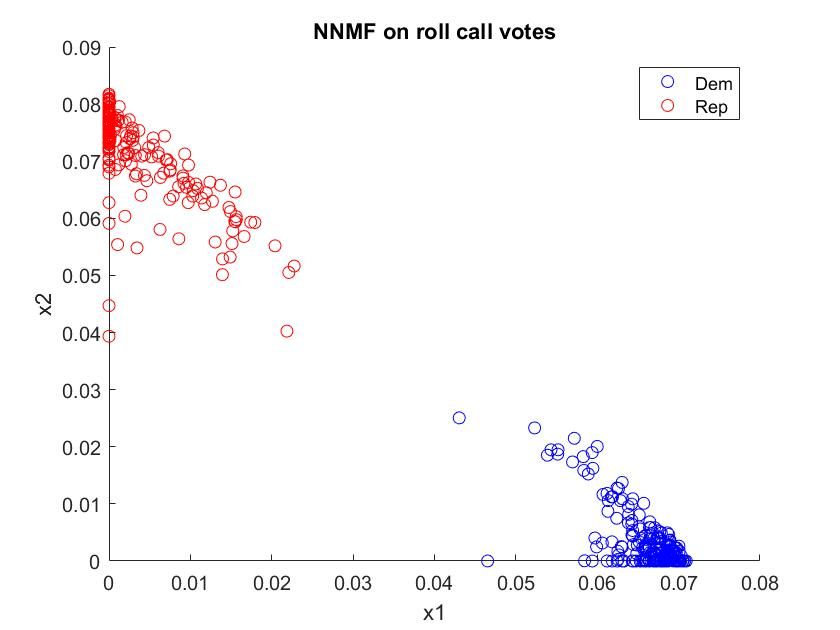
\includegraphics[width=\textwidth]{NNMF_votes.jpg}
        \caption{}
        \label{fig:NNMF}
    \end{subfigure}
          \begin{subfigure}[b]{0.4\textwidth}
        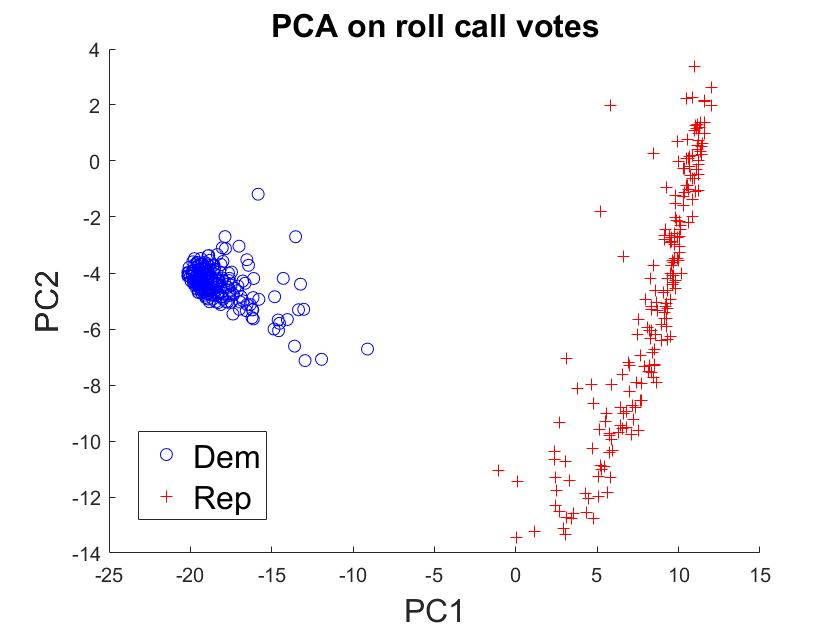
\includegraphics[width=\textwidth]{PCA_votes}
        \caption{}
        \label{fig:PCA}
    \end{subfigure}
  \caption{Dimensionality reduction on roll call vote data in the House of Representatives in the 110th Congres. (a) Nonnegative matrix factorization on the $448\times 1707$ matrix (448 representatives, 1707 bills) of roll call votes into two matrices of dimensions $448\times 2$ and $2\times 1707$. The rows of the $448\times 2$ matrices were plotted to visualize the distribution of representatives in a 2D space, and we clearly see division along party lines. (b) Principle component analysis on the roll call vote data. The eigenvalues and eigenvectors of the $448\times 448$ covariance matrix of representative voting data were computed, and each representative's voting profile was projected onto the space of the two eigenvectors with the two largest eigenvalues.}
  \label{fig:DimRedux}
\end{figure}

\subsection{Motivation} 

%In fact, even simple dimensionality reduction techniques on roll call data are able to uncover the political characteristics of individual representatives. For example, in figure \ref{fig:NNMF}, we factored the $448\times1707$ matrix representing the 448 representatives and their votes on 1707 bills into two nonnegative matrices of dimensions $448\times 2$ and $2\times 1707$ . Plotting the $448\times 2$ matrix where each row places a representative in a two dimensional space, we are able to clearly identify party affiliation. \par
%
%Another dimensionality technique we applied to visualize voting data was principle component analysis (figure \ref{fig:PCA}). We formed the principle components by computing the two largest eigenvalues and their respective eigenvectors on the $448\times 448$ covariance matrix of vote data, and each representative's voting profile was projected onto the space spanned by these principle components. Again, we clearly see differentiation along party lines. 


%Another common analysis of roll call votes that may potentially yield more subtle structures in legislative preferences is to conduct {\itshape ideal point modeling}. {\color{red} maybe the next sentences goes in the introduction \{} Here, a congressman and a bill is presumed to lie in a latent `'ideological space,'' where the probability of a ``yay'' or ``nay'' response is a function of the bill's position and the congressman's position. The congressman's position is known as an `'ideal point'' because his or her utility decreases as a bill's position deviates from this point. {\color{red} \}}
% In Gerrish and Blei 2011, ideal points of each representative was drawn from a zero mean Gaussian prior. In this paper, we aim to obtain better estimates of the representatives' ideal points, and to do so, we incorporate data from caucus memberships using a stochastic block model (see models below) because we hypothesize that sharing caucuses with other representatives influences a representative's voting behavior. 

We chose to model caucus memberships because initial exploratory data analysis suggested that caucus memberships are related to a legislator's voting behavior. Figure \ref{fig:VotesVsCaucus} plots the number of shared caucuses between two representatives against the proportion of bills on which they voted the same way, and we see that the more caucuses two members share, the more likely they are to vote the same way. 

\begin{figure}[h]
  \centering
        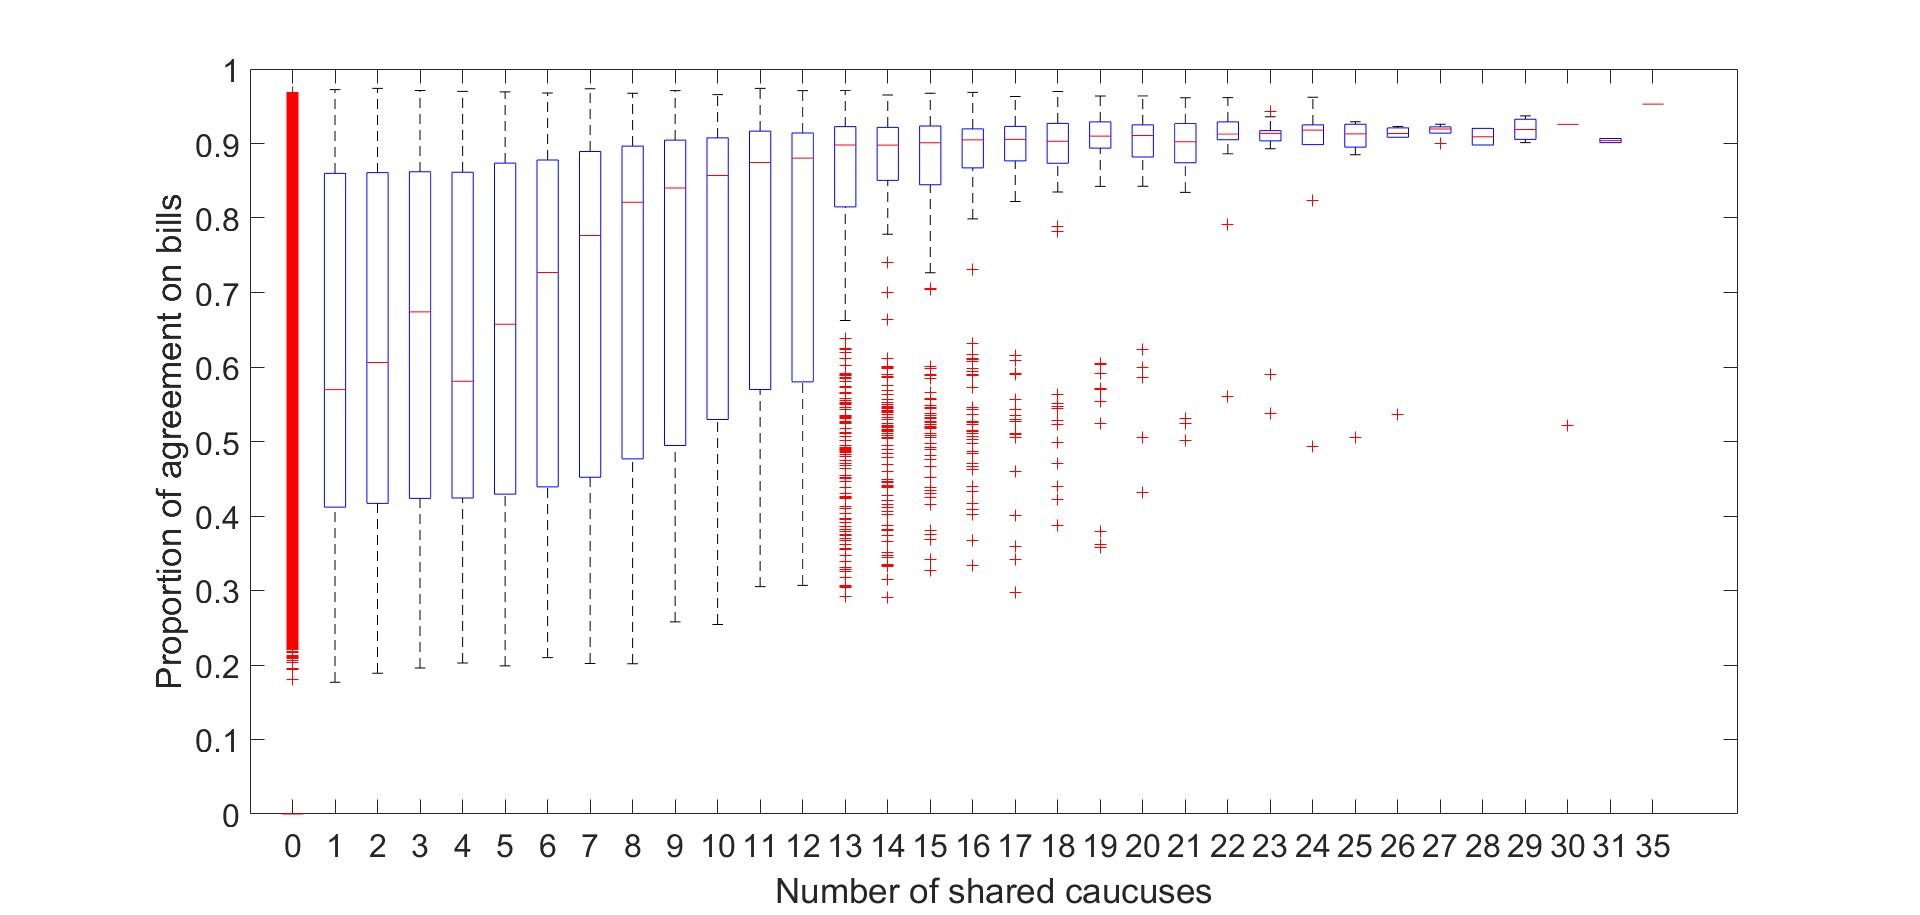
\includegraphics[width=\textwidth]{Caucus_vs_Votes.jpg}
  \caption{The distribution of agreement on bills as a function of the number of caucuses two representatives share. We see that the more caucuses people share, the more likely they are to agree on a bill. }
          \label{fig:VotesVsCaucus}
\end{figure}


Figure \ref{fig:Nhood_Caucus} shows the relationship between representatives within several caucuses in an undirected graphical model. We first used roll call vote data to infer the graph structure among the representatives in the entire House; we assumed pairwise interactions described via an Ising model in which each node denotes a binary variable of a representative voting either yes or no. The edges were inferred using neighborhood selection \cite{Hastie2015}, and the graphs shown in figure \ref{fig:Nhood_Caucus} are subsets of this full graph corresponding to members of a caucus. The connectivity (measured by the fraction of total edges present) of the full graph with 448 representatives is 0.064, while the connectivity within the caucus subgraphs was much higher. This suggests that a representative is more likely to be influenced by a member of his or her caucus than another random representative in the House.\par

Therefore, this strongly motivates taking into account interactions among the representatives in Congress. In particular, this analysis suggests that caucus memberships may at least partly explain whether two representatives will vote in a similar fashion. Therefore, we proceed in this project by utilizing caucus membership data and connecting them to ideal points using a stochastic block model; specifically, we hope that caucus memberships will inform a latent community structure among the representatives, and exploiting these interactions, we obtain better predictions of ideal points and hence better predictions of roll call votes. 

\begin{figure}[h]
  \centering
    \begin{subfigure}[b]{0.49\textwidth}
        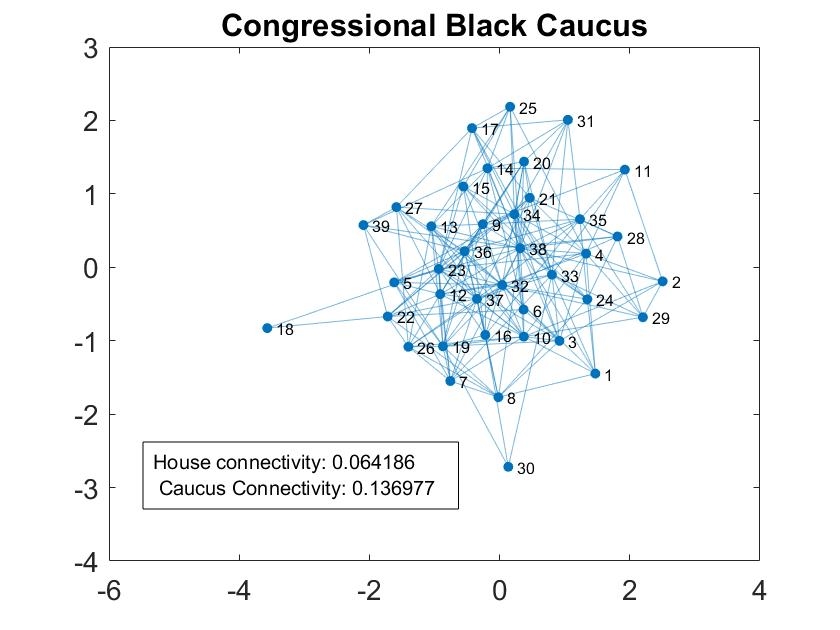
\includegraphics[width=\textwidth]{/Neighborhood_Regression/Congressional_Black_Caucus.jpg}
        \caption{}
    \end{subfigure}
          \begin{subfigure}[b]{0.49\textwidth}
        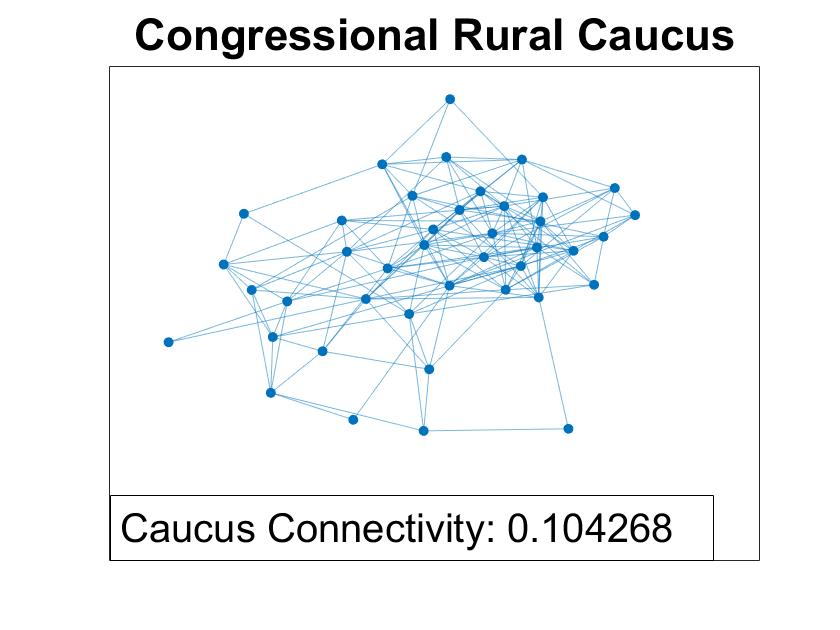
\includegraphics[width=\textwidth]{/Neighborhood_Regression/Congr_Rural_Caucus.jpg}
        \caption{}
    \end{subfigure}
        \begin{subfigure}[b]{0.49\textwidth}
        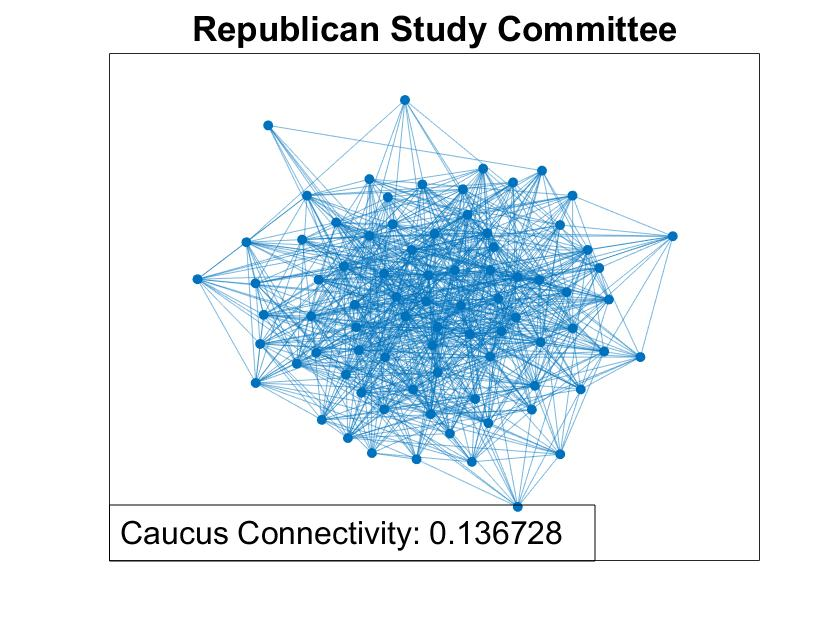
\includegraphics[width=\textwidth]{/Neighborhood_Regression/Rep_Study_Committee.jpg}
        \caption{}
    \end{subfigure}
          \begin{subfigure}[b]{0.49\textwidth}
        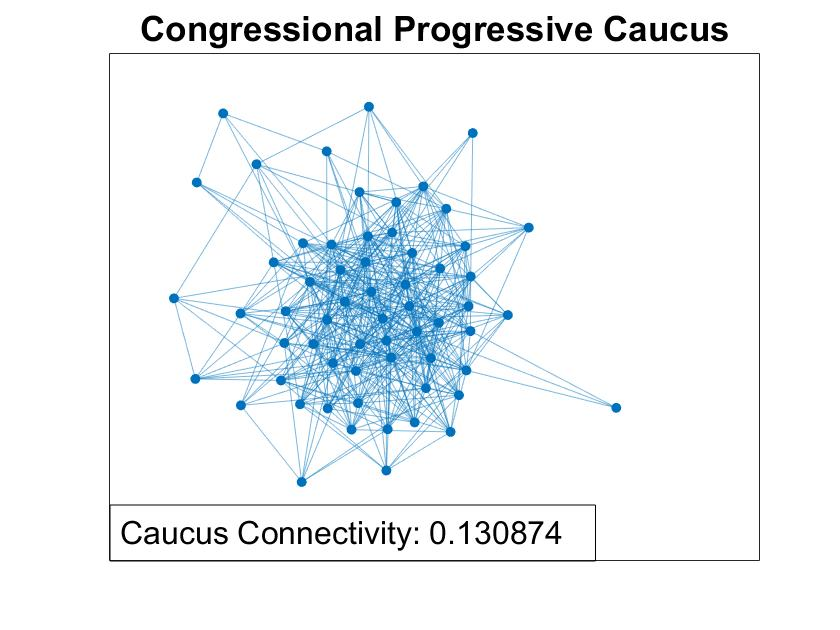
\includegraphics[width=\textwidth]{/Neighborhood_Regression/Congr_Prog_Caucus.jpg}
        \caption{}
    \end{subfigure}
  \caption{Neighborhood regression on roll call vote data was used to infer an undirected graphical model capturing relationships among all members of the House of Representatives. Each node represents a random variable corresponding to a legislator voting ``yea'' or ``nay'' on a bill, and we assumed pairwise interactions using an Ising model. Shown here are subgraphs with representatives taken from a given caucus. The caucuses are their connectivities shown here are (a) the Congressional Black Caucus, connectivity 0.137; (b) the Congressional Rural Caucus, connectivity 0.104; (c) the Republican Study Committee, connectivity 0.136; and (d) the Congressional Progressive Caucus, connectivity 0.131. In each case, the connectivity within the caucuses was higher than the connectivity of the full House (0.064).}
      \label{fig:Nhood_Caucus}
\end{figure}



\newpage


\section{Model}
\label{model}

\subsection{Ideal Point Model} 
The {\sl ideal point model} (IPM) \cite{Clinton2004} is a basic model for analyzing legislative behavior and revealed preferences with roll call voting data $(V_{ud})$ for a group of representatives $u$ voting on a collection of bills $d$. It assumes that each representative has a latent location $x_u\in\R^S$ called an {\sl ideal point}, and similarly that each bill has two vectors $a_d,b_d\in\R^S$, called the {\sl discrimination} and {\sl difficulty}, respectively. In quantitative political science, the ideal point $x_u$ is often treated as a proxy for one's ideological stance or preference. When $S=1$, the latent space may be considered a political spectrum. The discrimination $a_d$ quantifies how well votes on this bill separate liberals from conservatives: a bill $d$ is not discriminative $(a_d\approx 0)$ if representatives are largely indifferent to it. For discriminative bills, those representatives closest to the difficulty $b_d$ are likely to support it. A reasonable likelihood given these quantities is thus
\begin{equation}
V_{ud} \mid x_u, a_d, b_d \sim \text{Bern}(\sigma(a_d\cdot(x_u-b_d))).
\end{equation}
We place Gaussian priors over each of the latent variables:
\begin{equation}
a_d \sim \cn(\eta_{a},\sigma^2_{a}), ~~
b_d \sim \cn(\eta_{b},\sigma^2_{b}), ~~
x_u\sim \cn(\nu,\sigma^2_x),
\end{equation}
where the quantities $\eta_{a},\sigma^2_{a},\eta_{b},\sigma^2_{b},\nu,\sigma^2_x$ are fixed hyperparameters.

%For one, using it alone we can attempt to predict missing votes, a problem of interest in political science. Another problem of more qualitative interest is analyzing and interpreting the factors $a_d, b_d$ specific to a document and those $x_u$ specific to the representative. All are assumed to reside in some latent space $\R^S$ and so depending on how we set up the model, we might be able to interpret quantities like $x_u$ as $u$'s {\sl political stance} or {\sl ideological position} or $x_u - b_d$ as representative $u$'s propensity for the bill/document $d$. There are a number of problems we cannot address in IPM. A major problem is predicting on heldout documents (the `cold start'), which is a potentially useful performance measure. Similarly if we have relatively junior representatives, they may not have had enough votes for the inferred $x_u$ to represent something (1) meaningful / interpretable or (2) reliable. We want to incorporate more information to inform the choices of $a_d, b_d$ and $x_u$. We focus on the latter, with an interest in being able to better interpret the ideal points of the representatives. We use the stochastic block model to model the assumption that representatives `vote in groups' in the sense that they belong to various communities which tend to have the similar positions.


\subsection{Stochastic Block Model}

{\sl Stochastic block models} (SBM) \cite{Snijders1997} in general seek to model a graph---in our case, over $U$ representatives. Similar to the IPM, the SBM frames our understanding of the structure of our observations using latent variables. The latent variable $M_u\in\{1,\dots,K\}$ associated to representative $u$ designates to which of $K$ communities she belongs. The structure of the underlying graph specifies the probability of an interaction $R_{uv}$ between representatives $u$ and $v$. We assume $(R_{uv})$ contains counts for the number of interactions between $u$ and $v$ (commonly binary data is used instead). Our version of the SBM assumes the community assignments are i.i.d. draws from a pmf $\pi = (\pi_k)$ on $\{1,\dots,K\}$, and that each pair of communities $k,l\in\{1,\dots, K\}$ has co-expression rate $P_{kl}$. Our likelihood is
\begin{equation}
R_{uv} \mid P, M_u=k, M_v=l\sim \text{Poisson}(P_{kl}).
\end{equation}
To achieve conditional conjugacy, we assume $\pi \sim \text{Dir}(\gamma1_K)$ and $P_{kl} \simiid \text{Gamma}(\lambda_0,\lambda_1)$.


\subsection{Latent Community Ideal Point Model}

We relate the ideal points $x_u$ of IPM to the relational data $(R_{uv})$ using a stitching together of the two models described above, which we call the {\sl latent community ideal point model} (LC-IPM). We introduce $K$ community ideal points $\nu_k\simiid\cn(\varpi,\sigma^2_\nu)$. The ideal point $x_u$ now follows a normal distribution centered around its community mean $\nu_{M_u}$. LC-IPM simultaneously models for the voting data $(V_{ud})$ and the relational data $(R_{ud})$. The graphical model is provided below.


\begin{figure}[h]
  \centering
        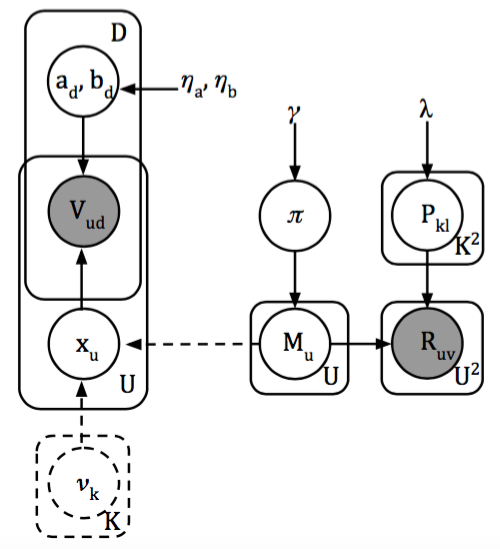
\includegraphics[width=12em]{lcipm2.png}
  \caption{Graphical model for LC-IPM. Left: ideal point model. Right: stochastic block model.}
      \label{fig:pgm}
\end{figure}

\subsection{Related Work}

Bayesian methods for ideal point modeling have become an important tool in analyzing revealed preferences in government \cite{Clinton2004}. Previously these methods have been extended to consider the discrimination $a_d$ and difficulty $b_d$ as response variables with covariates related to the topical content of the bill using {\sl supervised latent Dirichlet allocation} \cite{Gerrish2011}. Relating the posterior of $a_d$ and $b_d$ to the text of the bill (in addition to the votes) addresses the {\sl cold start problem}, i.e. the ability to predict votes on new bills. We adopt a similar approach, where the ideal points $x_u$ for representatives with limited voting data can lean on the community mean $\nu_{M_u}$. Both methods are more broadly applicable to collaborative filtering for behavior data when related data sources are present. Previous analyses have performed SVD on roll call voting data to reveal correlations in political structure and latent community structure \cite{Porter2007}.

\section{Posterior Inference}
\label{inference}

Upon observing votes $V = (V_{ud})$ and caucus co-membership counts $R = (R_{uv})$, computing the posterior distribution of the latent variables given the observations
$$
p(x, a, b, \pi, P, M \mid V, R)
$$
 is intractable. We employ {\sl na\"ive mean field variational inference}, finding the distribution $q$ closest in KL divergence to the posterior among all fully factorized distributions. Minimizing the KL divergence is equivalent to maximizing the evidence lower bound (ELBO):
\begin{align*}
\cl(q)
&= \EE_q\left[\log \frac{p(\nu, x, a, b, \pi, P, M, V, R)}{q(\nu, x, a, b, \pi, P, M)}\right] \\
&= \EE_q\left[\log \frac{p(a, b, V)p(x\mid M, \nu)p(\nu)}{q(\nu)q(x)q(a)q(b)}\right]
+ \EE_q\left[\log \frac{p(\pi, P, M, R)}{q(\pi)q(P)q(M)}\right].
\end{align*}
Each factor of $q$ follows a simple parametric form, described in appendix \ref{vi}. The simplest approach to variational inference maximizes the ELBO $\cl(q)$ via coordinate-ascent, choosing the best value of a variational parameter with all others fixed. Iteratively applying these updates, the variational approximation $q$ improves at every step toward some local optimum. Conditional conjugacy yields closed form updates for the variational parameters corresponding to $\pi$ and $P$ \cite{Blei2016}. Furthermore, due to the decomposition of the ELBO $\cl(q)$ above, the mean field factorization yields the same variational updates for $\pi, P, a_d$, and $b_d$ as in SBM and IPM, and we exploited this modularity. We devised our implementation of coordinate-ascent variational inference (CAVI) for IPM, SBM, and LC-IPM to have as little repeat code as possible by defining LC-IPM as a class which extends from both of its component parts. 


\newpage

\section{Empirical Results}
\label{results}
To evaluate the performance of LC-IPM we attempted to recover known model parameters from simulated data; we also evaluated the model's predictive performance on data from the 110\textsuperscript{th} congress. For the following results we implemented CAVI for LC-IPM in Python \footnote{Implementation can be found at \url{www.github.com/ebenmichael/congress-bills}}
\subsection{Simulated Data}
\begin{figure}[h]
  \centering
    \begin{subfigure}[b]{0.3\textwidth}
        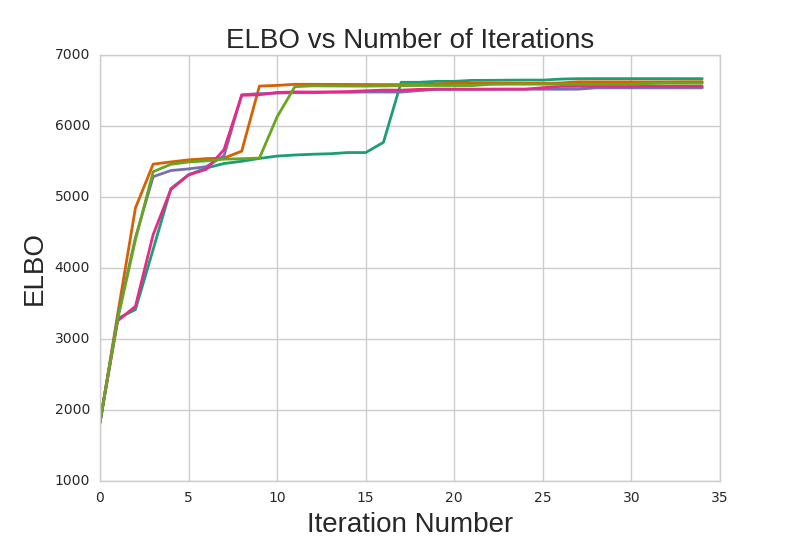
\includegraphics[width=\textwidth]{toy_elbos.png}
        \caption{}
    \end{subfigure}
          \begin{subfigure}[b]{0.3\textwidth}
        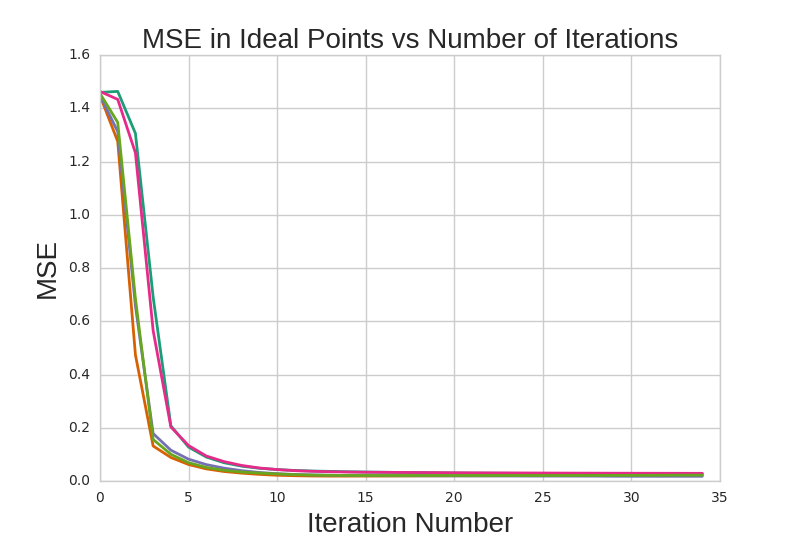
\includegraphics[width=\textwidth]{toy_ip_mse.png}
        \caption{}
    \end{subfigure}
        \begin{subfigure}[b]{0.3\textwidth}
        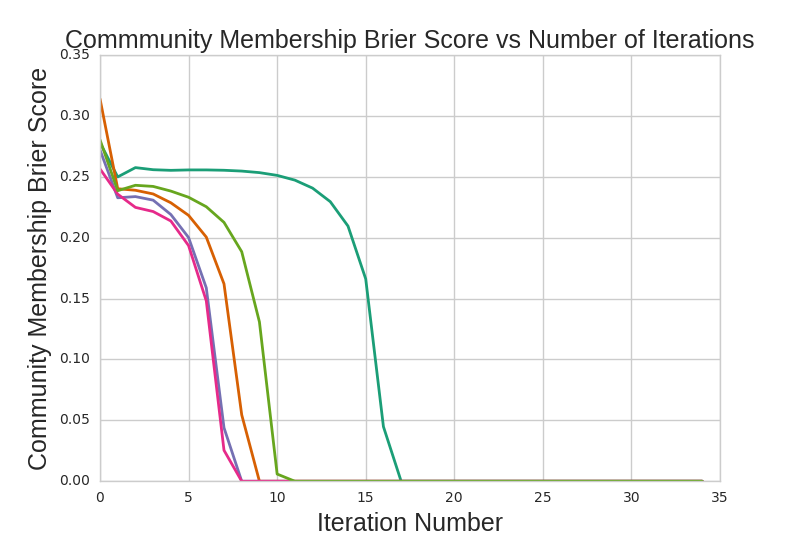
\includegraphics[width=\textwidth]{toy_resp_mse.png}
        \caption{}
    \end{subfigure}
  \caption{(a) ELBO (b) MSE between posterior mean ideal points and true ideal points and (c) Brier score between posterior mean community assignments and true assignments vs number of CAVI iterations on simulated data for 5 random data sets generated from the model}
      \label{fig:toy_results}
\end{figure}

To ensure that CAVI produces reasonable posterior inferences, we sampled vote interactions and caucus co-membership counts from the generative model and compared the true model parameters to the naive mean field approximation. We generated 50 representatives, 500 documents, and two communities, using one dimensional ideal points and ran the CAVI routine for 35 iterations. To evaluate convergence we output the ELBO at each iteration. To evaluate the approximate posterior means we compared the variational ideal point mean $\hat{\tau}_u$ to the true ideal point $x_u$ for each representative and the posterior responsibility of the first community $\hat{r}_{u1}$ to the true community assignment $M_u$ with the Mean Square Error (MSE) and Brier Score (Brier):
\begin{align*}
 \text{MSE}(x, \hat{t}) = \frac{1}{U} \sum_{u=1}^U (x_u - \hat{\tau}_u) ^2  \;\; & \;\; \text{Brier}(\hat{r}_1, M) = \frac{1}{U} \sum_{u=1}^U (M_u - \hat{r}_u)^2
\end{align*}
Because the model is invariant to permutations of the communities and reflections of the ideal points, we chose the permutation and reflection which minimized the scores. We ran this analysis on 5 different data sets generated according to the model; the results of this experiment are in Figure \ref{fig:toy_results}. We see that CAVI very quickly converges to the correct ideal points while taking longer to converge to the correct community assignments. Overall the mean square error is close to zero and the naive mean field approximation recovers the correct parameters.
\subsection{110\textsuperscript{th} Congress}
\subsubsection{Data}
We obtained roll call vote records for the House of Representatives of the 110\textsuperscript{th} Congress from \href{www.govtrack.us}{GovTrack.us}, an independent open government data website which publishes and stores data related to the United States Congress. Our data set contains 1707 documents (those categorized as bills, amendments, and motions) and 448 representatives. We only consider those roll call votes where a representative voted \texttt{yea} or \texttt{nay}; there were 703,830 such interactions. We gathered caucus membership data from \cite{Victor2013}.
\subsubsection{Evaluation} 
To evaluate our model we assess predictive accuracy. We compared a $K=2$ community and $K=10$ community LC-IPM with dimension $S=2$ with predicting \texttt{yea} each time (Yea), $L^2$ regularized Logistic Regression, and the standard Ideal Point Model with dimension $S=1$ and $S=2$. We first chose the regularization parameter for Logistic Regression using a 5 fold cross validation procedure. We performed another 5 fold cross validation procedure where we trained each model on 4 folds, tested on the 5\textsuperscript{th} validation fold, and averaged the results; Table \ref{table:results_table} has these results. We found that LC-IPM and IPM both perform very well and roughly the same.

\vspace{2ex}
\begin{table}
\begin{center}
\begin{tabular}{c | c |c}
Model &  Accuracy & AUC\\ %$\sigma^2_x$&
\hline
\hline
Yea & 67.123 & 50.000\\
Logistic Regression & 78.340 & 85.105\\
\hline
IPM ($S= 1$)  &  94.769 & 98.418\\
IPM ($S= 2$)  & 95.451 & 98.998\\
\hline
LC-IPM ($S=2, K=2$)  & 95.405 & 99.013\\
LC-IPM ($S=2, K=10$)  & 95.415 & 99.015
\end{tabular}
\end{center}
\caption{Averaged held out test set prediction metrics}
\label{table:results_table}
\end{table} 

\subsubsection{Inferred Ideal Points and Communities}
In this section we examine inferred ideal points and communities from the House of Representatives in the 110\textsuperscript{th} Congress.


\begin{figure}[h]
  \centering
    \begin{subfigure}[b]{0.45\textwidth}
        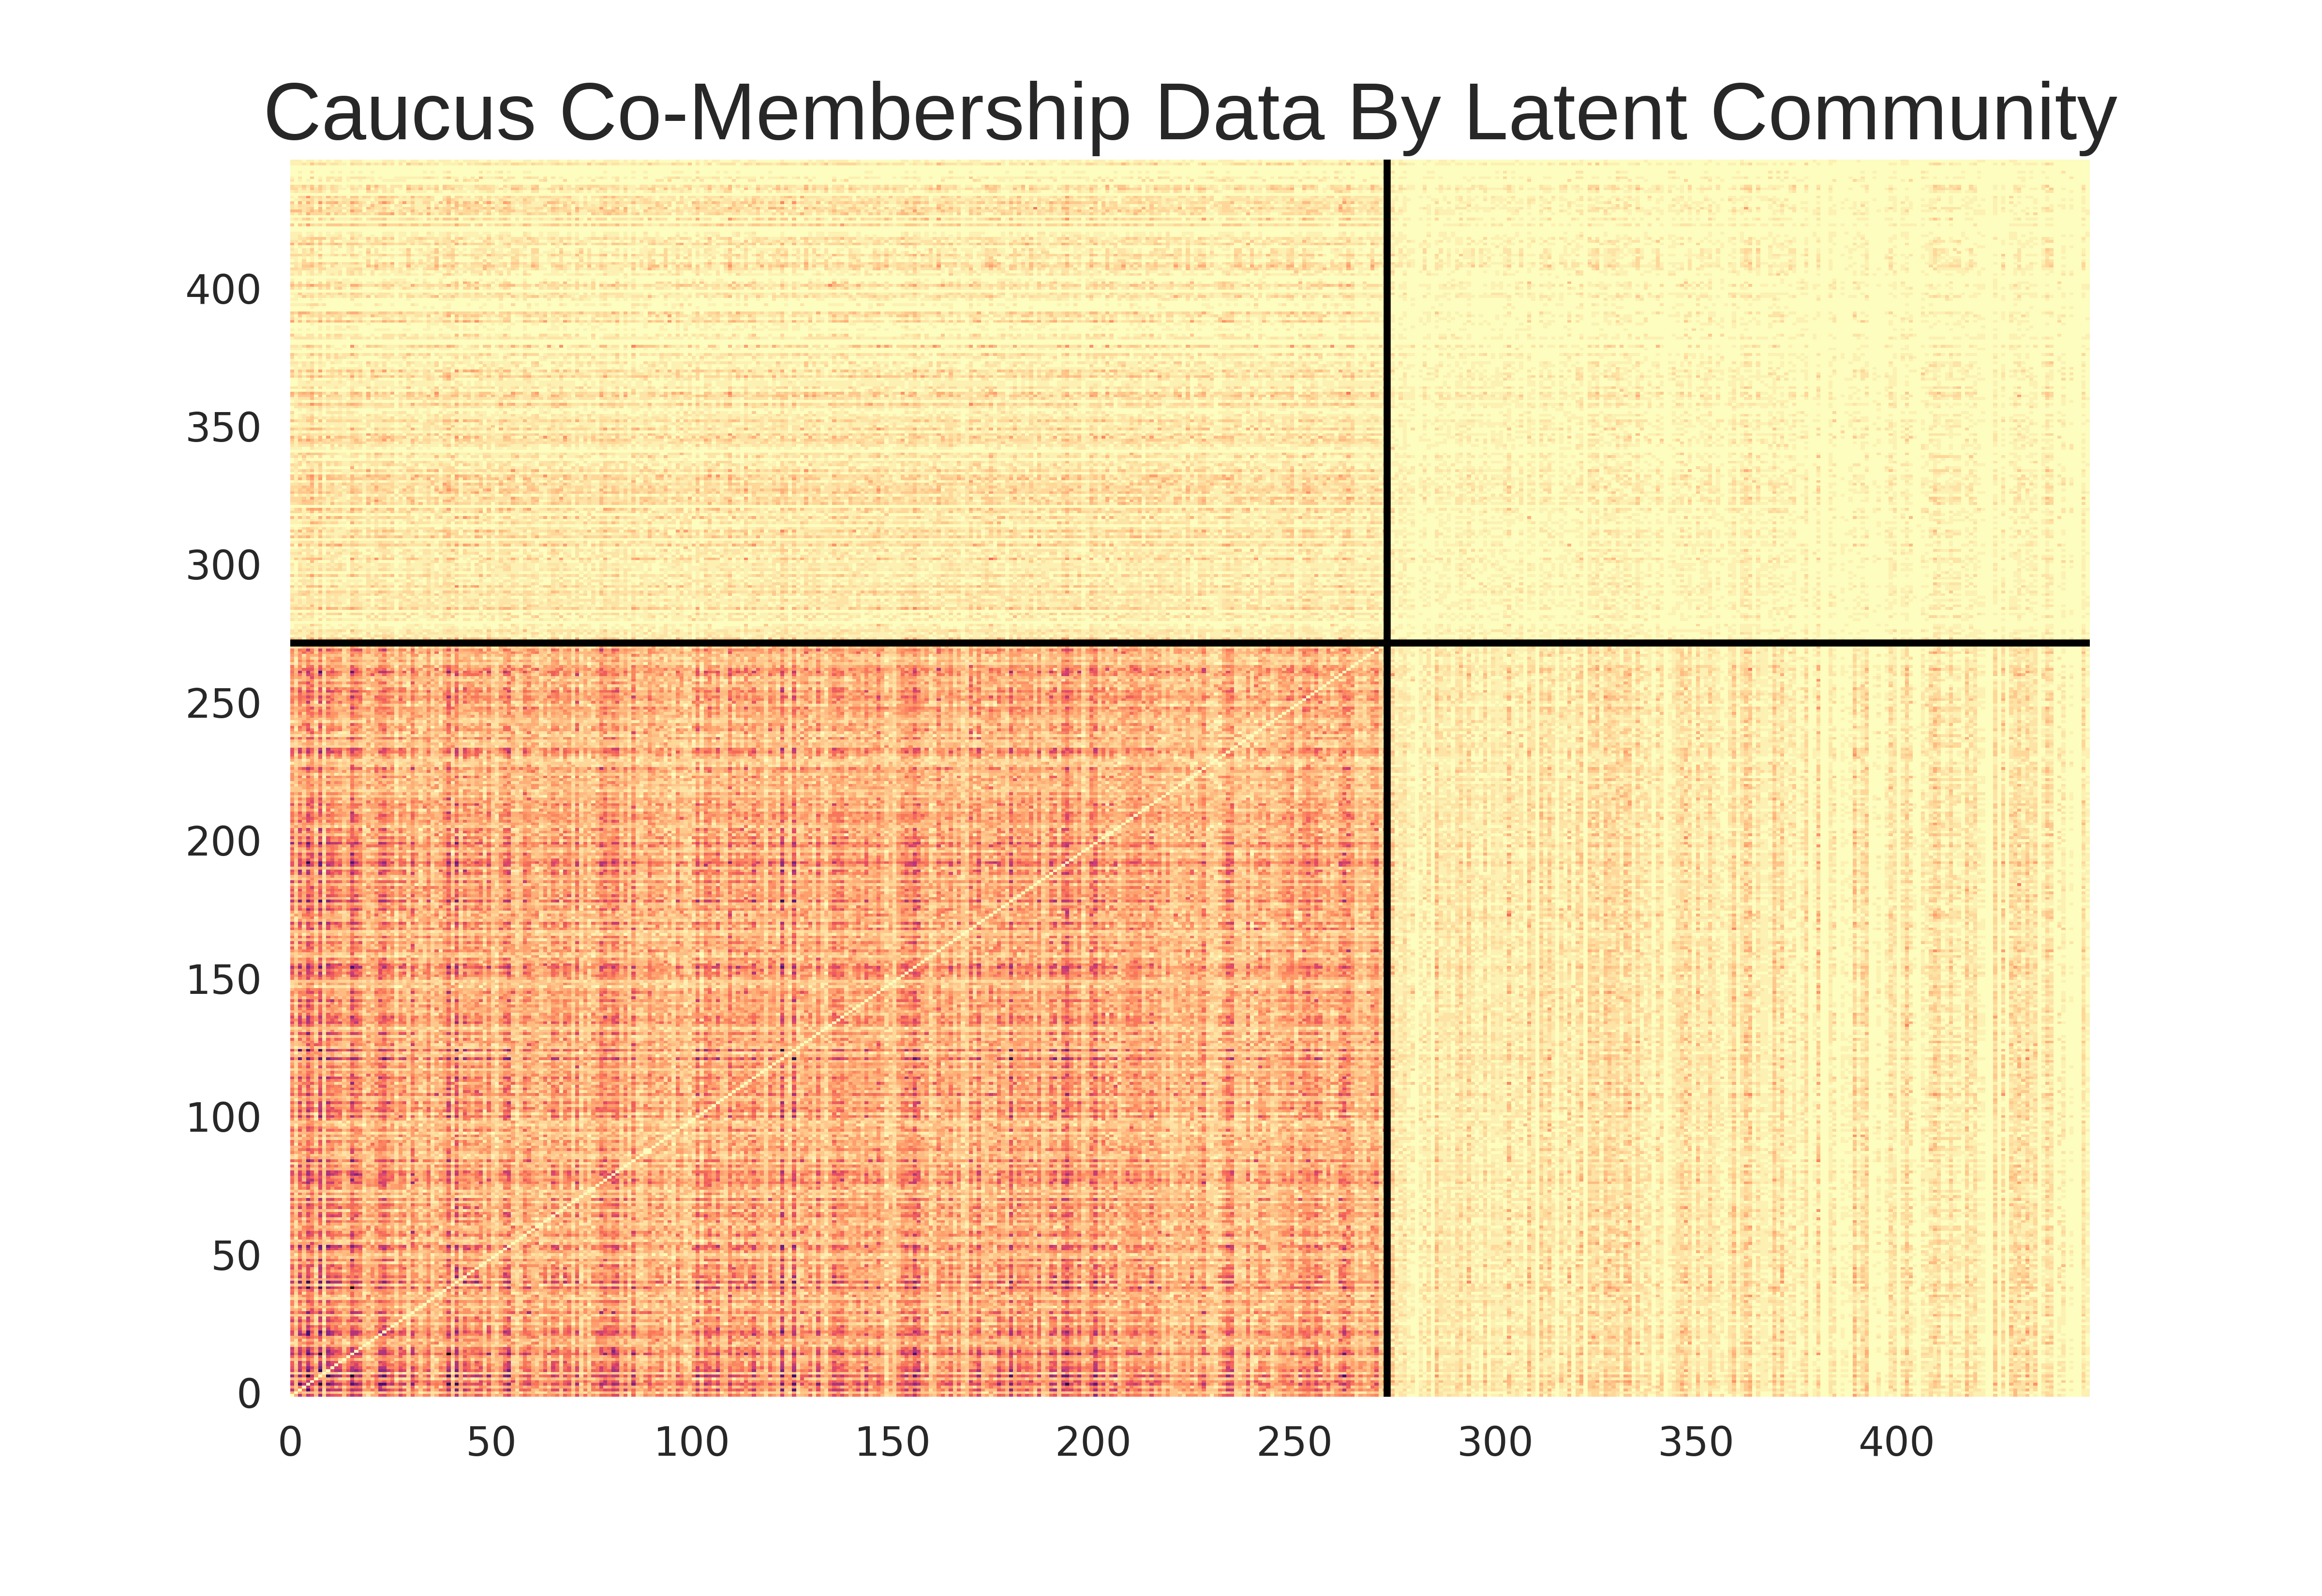
\includegraphics[width=\textwidth]{2_communities.png}
        \caption{}
    \end{subfigure}
    \begin{subfigure}[b]{0.45\textwidth}
        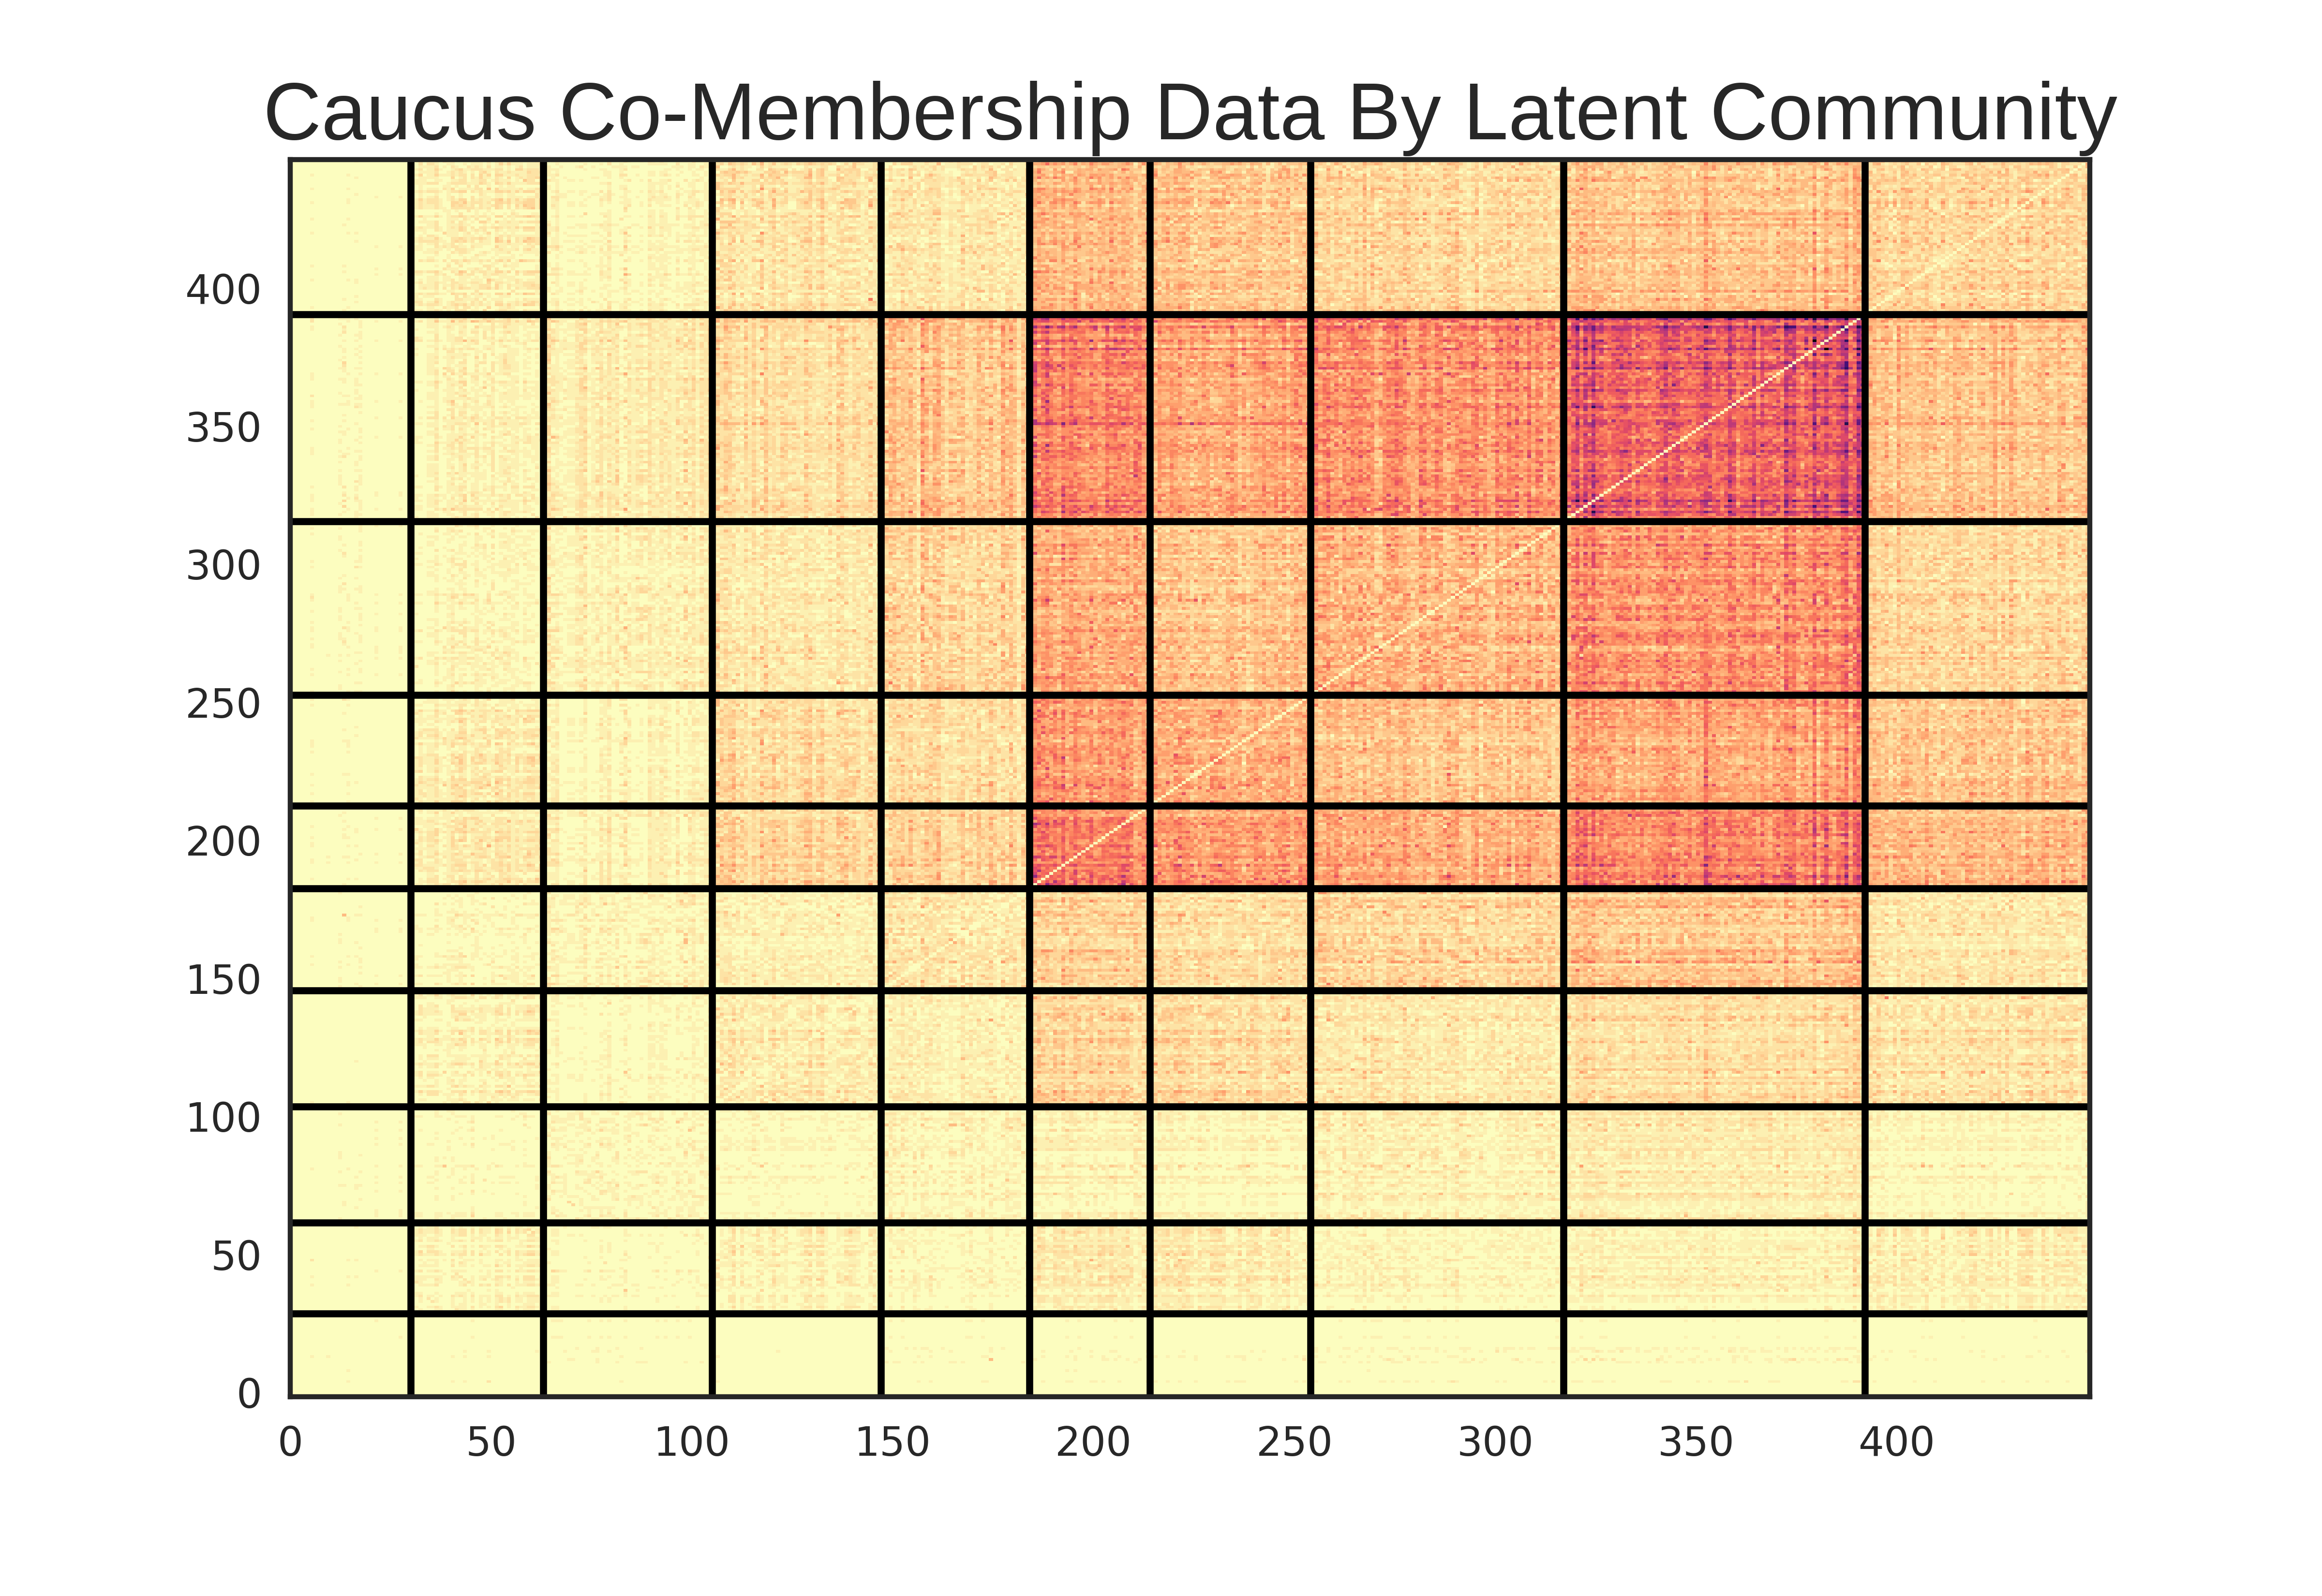
\includegraphics[width=\textwidth]{10_communities.png}
        \caption{}
    \end{subfigure}

  \caption{Caucus co-membership counts grouped by inferred community for (a) 2 and (b) 10 communities. Each entry denotes the number of caucuses shared by a pair of representatives. Red denotes many (up to thirty) common caucuses; yellow denotes close to no common caucuses. The 10 community model captures finer block structure.}
      \label{fig:2_comm_lcipm}
\end{figure}

\begin{figure}[h]
  \centering
          \begin{subfigure}[b]{0.45\textwidth}
        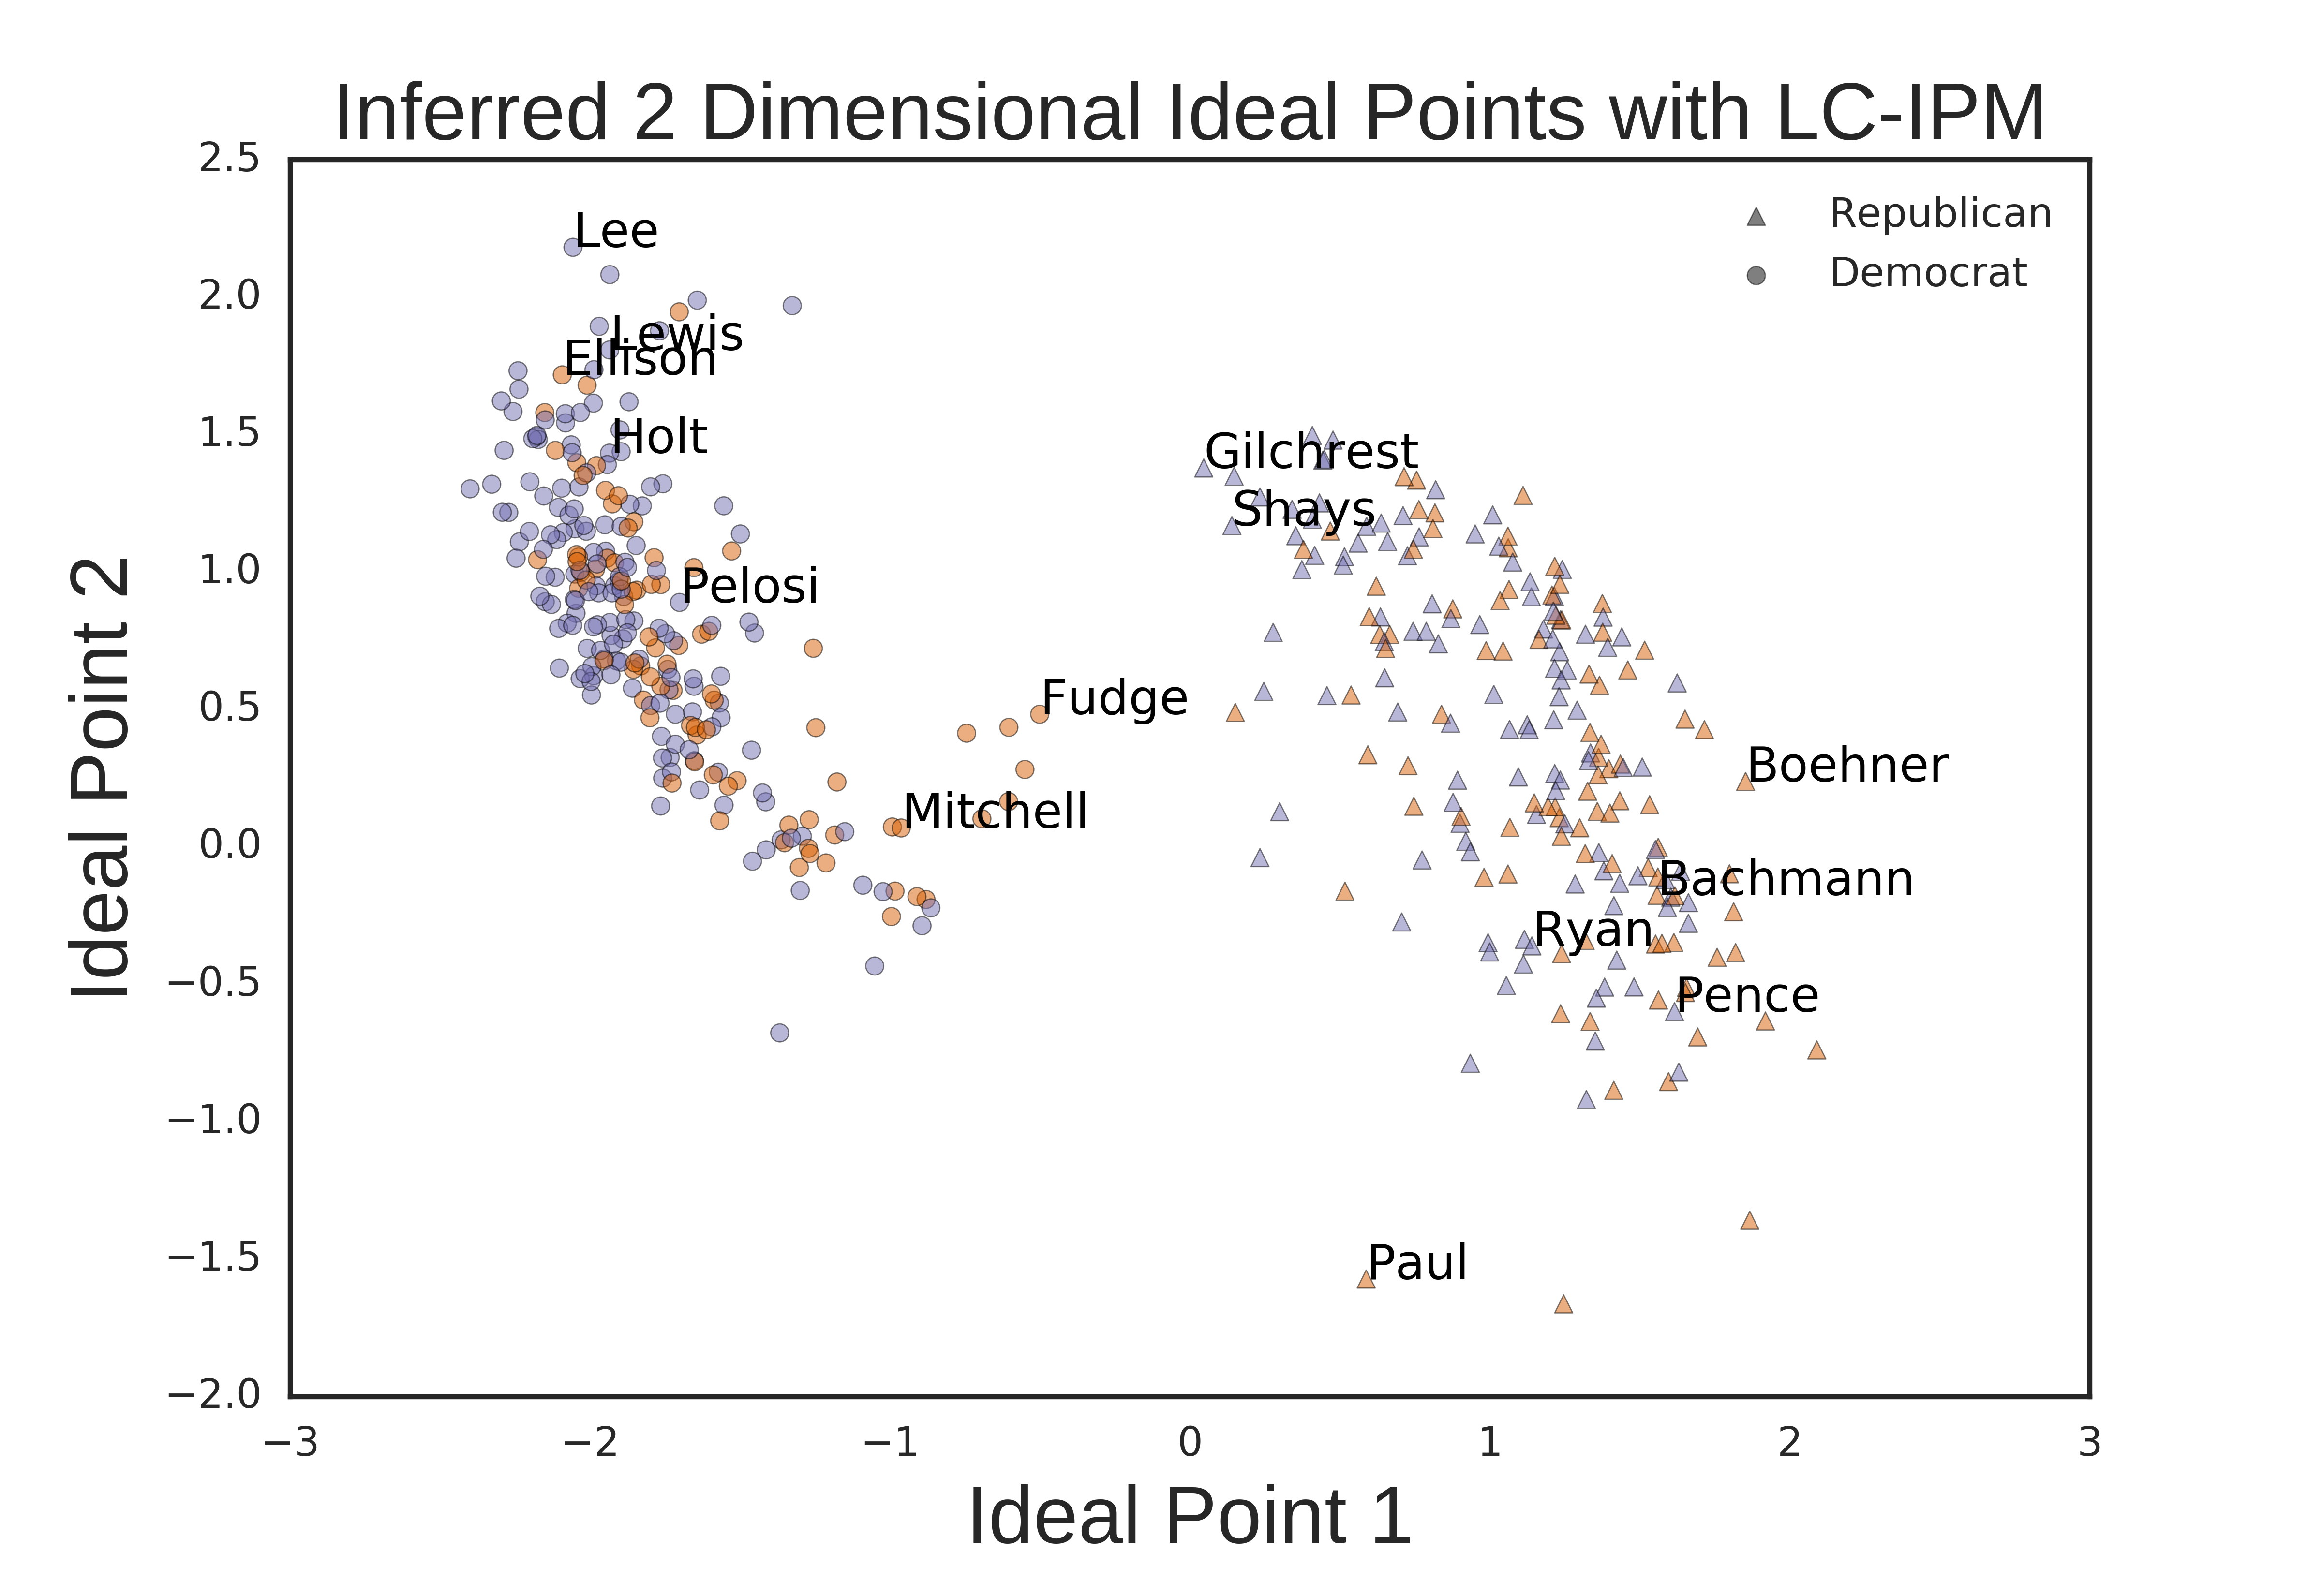
\includegraphics[width=\textwidth]{ideal_points_congress_2.png}
        \caption{}
    \end{subfigure}
          \begin{subfigure}[b]{0.45\textwidth}
        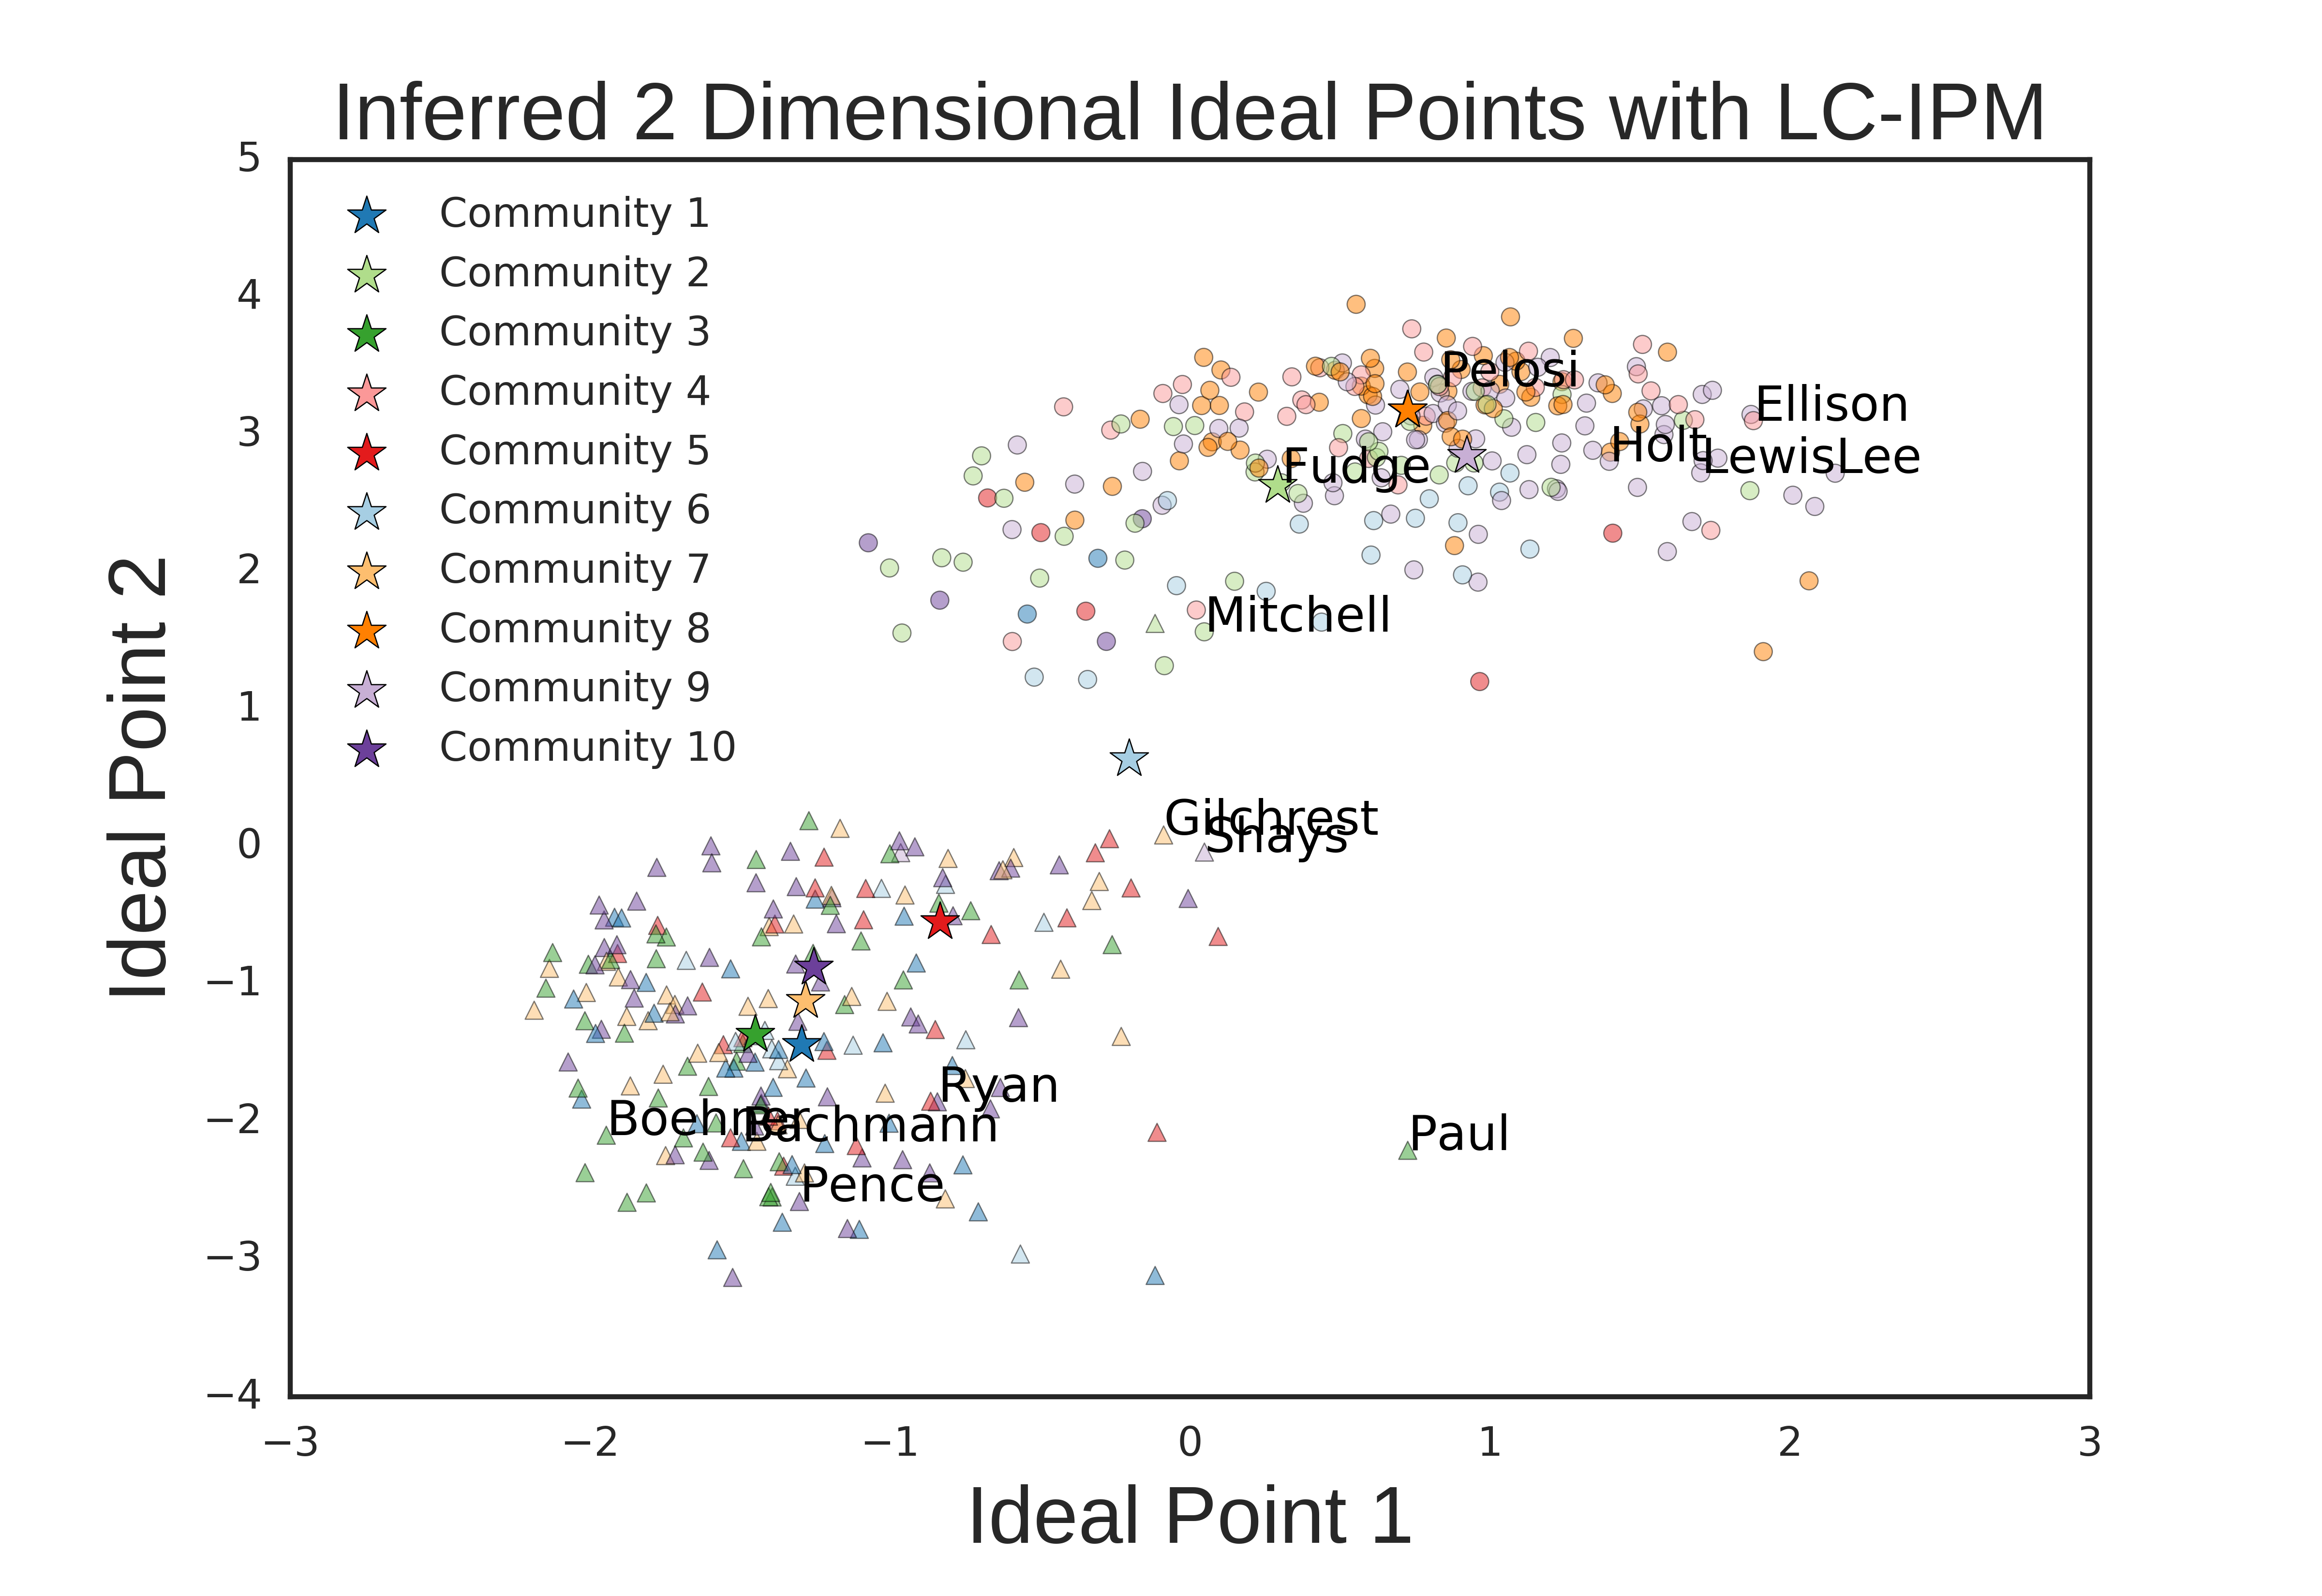
\includegraphics[width=\textwidth]{ideal_points_congress_10.png}
        \caption{}
    \end{subfigure}

  \caption{Inferred 2 dimensional ideal points for an LC-IPM model with (a) 2 and (b) 10 communities. Shape denotes party affiliation; color denotes community; stars in (b) indicate inferred community means. Both models separate Republicans and Democrats with noted centrists in between.}
      \label{fig:2_comm_lcipm}
\end{figure}

We first ran CAVI on an LC-IPM model with dimension $S=2$ and $K=2$ communities. With this configuration the ideal points are well separated by party (Figure \ref{fig:2_comm_lcipm} b) but the inferred communities straddle party lines. We sorted the raw caucus co-membership counts by inferred community and found that there is one community where members share a large number of caucuses, and another where the members do not share very many caucuses (Figure \ref{fig:2_comm_lcipm} a). Running CAVI on an LC-IPM model with dimension $S=2$ and $K=10$ communities retains the clean separation by party and overall shape of the ideal points (noting that the model is invariant to rotations). However, the community structure is markedly different. The inferred communities simultaneously capture fine block structure in the caucus co-membership counts and inter and intra party spatial structure of the ideal points. 

The concurrent relational and spatial models allow for interesting conclusions. For instance, we can see that the 9\textsuperscript{th} community has a high rate of caucusing together and is comprised of Democrats with ideal points far from Republicans and centrists, leading to an interpretation that the 9\textsuperscript{th} community is a strongly interconnected group of staunch liberals. The four depicted members of this community (Rush Holt, Keith Ellison, John Lewis, and Barbara Lee) are regarded as very liberal representatives. We can also see representatives such as centrist Wayne Gilchrest, who broke ranks with the Republican party more often than any other representative in 2007, libertarian Ron Paul, who challenges Republican social policy, who are in communities which nonetheless are deeply conservative.

\section{Conclusions and future directions} 
While LC-IPM offers similar predictive performance to the standard ideal point model, we gain the ability to detect more subtle clusters within and between the two large party clusters. This ability to analyze the social network among members of Congress is of particular interest to political scientists. \par

Moreover, by taking into account caucus data, we can still make reasonable predictions for junior representatives for whom we do not have extensive vote data.  {\color{red} Eli will add to this}  \par

Finally, a key advantage to our generative model is its modularity, and in future work we would be interested in the composability of hierarchical models from multiple data sources. While this project incorporated caucus data to better inform estimates for the representatives' ideal points, another direction to explore would be to utilize data on bills to better estimate their difficulty and discrimination. For example, we may follow the example in \cite{Gerrish2011} to combine LC-IPM with supervised topic modeling and infer the latent topics in a bill from a bill's text; these latent topics then inform a bill's difficulty and discrimination. On the other hand, we may also explore incorporating legislators' speech transcripts in deliberating the bill (\cite{Quinn2006}, \cite{Thomas2006}). Our model could also be augmented by incorporating bill metadata (like sponsorships), or legislator metadata (like ethnicity or state). \par

Overall, LC-IPM connects voting data to caucus memberships, and enables us to analyze how a social network influence legislative results. While we were motivated by congressional data, our model also applies to more general collaborative filtering settings with relational data.

\iffalse
\section{Contributions}
\begin{itemize}
\item Bryan: pca, nbhd regression, section \ref{introduction} of writeup.
\item Jake: SBM, sections \ref{model}, \ref{inference}, \ref{discussion} and \ref{sbmvi} of writeup.
\item Eli: dataset, IPM, experiments, sections \ref{results} and \ref{ipmvi} of writeup.
\item Collectively: section \ref{lcipmvi} of writeup, poster
\end{itemize}
\fi

\newpage



%[1] Gerrish, S.M.\ \& Blei, D.M. \ (2011) Predicting Legislative Roll Calls from Text. {\it Proceedings of the 28th International Conference on Machine Learning}
%\noindent[1] Wainwright, M. J. \& Jordan, M. I. (2008). Graphical models, exponential families, and variational inference. {\sl Foundations and Trends in Machine Learning}. \\
%
%\noindent[2] Gerrish, S. M. \& Blei, D. M.  (2011). Predicting legislative roll calls from text. {\it Proceedings of the 28th International Conference on Machine Learning}. \\
%
%\noindent[3] Blei, D. M., Kucukelbir, A. \& McAuliffe, J. D. (2016). Variational inference: a review for statisticians. {\sl arXiv:1601.00670}.

\begin{thebibliography}{10}

\bibitem{Blei2016} Blei, D. M., Kucukelbir, A. \& McAuliffe, J. D. (2016). Variational inference: a review for statisticians. {\sl arXiv:1601.00670}.

\bibitem{Braun2010} Braun, M. \& McAuliffe, J. (2010). Variational inference for large-scale models of discrete choice. {\itshape Journal of the American Statistical Association}. 105(489): 324-334. 

\bibitem{Clinton2004} Clinton, J., Jackman, S. \& Rivers D. (2004). The statistical analysis of roll call data. {\itshape American Political Science Review}. 98(2): 353-370. 

\bibitem{Gerrish2011} Gerrish, S.M. \& Blei, D.M. (2011) Predicting legislative roll calls from text. {\it Proceedings of the 28th International Conference on Machine Learning}.

\bibitem{Hastie2015} Hastie, T. J., Tibshirani, R. \& Wainwright, M. J. (2015). Statistical learning with sparsity: the Lasso and generalizations. {\itshape CRC Press}. 

\bibitem{Porter2007} Porter, M. A., Mucha, P. J., Newman, M. E. J. \& Friend, A. J. (2007). Community structure in the United States House of Representatives. {\it Physica A}.

\bibitem{Quinn2006} Quinn, K M., Monroe, B L., Colaresi, M., Crespin, M H. \& Radev, D R. (2006). An automated method of topic-coding legislative
speech over time with application to the 105th-
108th u.s. senate. {\itshape In In Midwest Political Science
Association Meeting}

\bibitem{Snijders1997} Snijders, T. A. B. \& Nowicki, K. (1997). Estimation and prediction for stochastic blockmodels for graphs with latent block structure. {\itshape Journal of Classification}.

\bibitem{Thomas2006} Thomas, M., Pang, B. \& Lee, L. (2006). Get out
the vote: Determining support or opposition from
congressional floor-debate transcripts. {\itshape Proceedings
of EMNLP}. 327–335.

\bibitem{Wainwright2008} Wainwright, M. J. \& Jordan, M. I. (2008). Graphical models, exponential families, and variational inference. {\sl Foundations and Trends in Machine Learning}. 

\end{thebibliography}

\appendix

\newpage

\section{Variational updates}

\subsection{Stochastic Block Model (SBM)}
\label{sbmvi}

After observing the symmetric matrix $R = (R_{uv})$, where $R_{uv}$ is the number of caucuses that representatives $u$ and $v$ have in common, we see to find a distribution $q$ over the latent community assignments $M = (M_u)$, the community coexpression rates $P = (P_{kl})$, and the community proportions $\pi = (\pi_k)$ which is close in relative entropy to the true posterior and lies in the factorized family $q(M)q(P)q(\pi)$. Each factor has free parameters described below and denoted with $\widehat{\text{hats}}$. The approximation $q$ is equivalently scored by the ELBO objective $\cl$, which we break down as:%arrange into component terms:
\begin{equation*}
\begin{split}
\cl(q)
%&= \EE_q\left[\log\frac{p(R,M,P,\pi)}{q(M,P,\pi)}\right]  \\
&= \underbrace{\EE_q\left[\log p(R\mid M,P)+ \log\frac{p(P)}{q(P)}\right]}_{\cl_{\text{data}}}
+ \underbrace{\EE_q\left[-\log q(M)\right]}_{\cl_{\text{ent}}}
+ \underbrace{\EE_q\left[\log p(M\mid \pi)\right]}_{\cl_{\text{local}}}
+ \underbrace{\EE_q\left[\log\frac{p(\pi)}{q(\pi)}\right]}_{\cl_{\text{global}}}
\end{split}
\end{equation*}
~\vspace{-1em}

\noindent{\bf Variational Factors.} To each $u$ we associate variational parameters $\widehat r_u = \left(\widehat r_{uk}\right)_{k=1}^K$, so
\begin{align}
q(M) = \prod_{u=1}^U q(M_u\mid \widehat r_u) 
= \prod_{u=1}^U \prod_{k=1}^K \widehat r_{uk}^{\delta_k(M_u)}.
\end{align}
We define 
$q(\pi) \triangleq \text{Dir}(\widehat \gamma_1, \dots, \widehat \gamma_K)$ and $q(P) \triangleq \prod_{kl}\text{Gamma}(\widehat \lambda_{0kl},\widehat \lambda_{1kl})$. %where $q(P_{kl}\mid \widehat \lambda_{kl})\triangleq \text{Gamma}(\widehat \lambda_{kl})$. \\

\noindent{\bf Computing the ELBO.} Now we can write out the component terms of the ELBO more explicitly:
\begin{equation*}
\begin{split}
\cl_{\text{data}}
&= \EE_q\left[\log p(R\mid M,P)+ \log\frac{p(P)}{q(P)}\right]
= \sum_{kl}\EE_q\left[\sum_{u,v}\delta_{k}(M_u)\delta_l(M_v)\log p(R_{uv}\mid P_{kl})+ \log\frac{p(P_{kl})}{q(P_{kl})}\right] \\
&= -\sum_{u,v}\log R_{uv}! + \sum_{k,l} \left(\lambda_{0}\log\lambda_1-\widehat\lambda_{0kl}\log\widehat\lambda_{1kl} - \log\frac{\Gamma(\lambda_0)}{\Gamma(\widehat\lambda_{0kl})}\right) + \sum_{k,l} \cl_{kl}(R)
~\\
\cl_{\text{ent}}
&= \EE_q\left[-\log q(M)\right]
= -\sum_{u,k}\EE_q\left[\delta_{k}(M_u)\log \widehat r_{uk}\right]
= -\sum_{u,k}\widehat r_{uk}\log \widehat r_{uk}
~\\
\cl_{\text{local}}
&= \EE_q\left[\log p(M\mid \pi)\right]
= \sum_{u,k}\EE_q\left[\delta_{k}(M_u)\log \pi_k\right]
= \sum_{k}N_k\EE_q\left[\log \pi_k\right]
~\\
\cl_{\text{global}}
&= \EE_q\left[\log\frac{p(\pi)}{q(\pi)}\right]
= \log \Gamma(C\gamma) - C\log\Gamma(\gamma) -\log \Gamma\left(\sum_k\widehat\gamma_k\right) + \sum_k\left\{\log\Gamma(\widehat\gamma_k)+ (\gamma-\widehat\gamma_k)\EE_q\left[\log \pi_k\right]\right\}
\end{split}
\end{equation*}
where $N_k = \sum_{u}\widehat r_{uk}$, $N_{kl} = \sum_{uv}\widehat r_{uk}\widehat r_{vl}$, $S_{kl} = \sum_{uv}\widehat r_{uk}\widehat r_{vl} R_{uv}$, and 
$$
\cl_{kl}(R) 
= (S_{kl} + \lambda_{0} - \widehat\lambda_{0kl}) \EE_q[\log P_{kl}]
   -(N_{kl} + \lambda_{1} - \widehat\lambda_{1kl}) \EE_q[P_{kl}], 
$$
and the posterior expectations can also be computed explicitly as 
$$
\EE_q[P_{kl}] =  \frac{\widehat\lambda_{0kl}}{\widehat\lambda_{1kl}}, ~
\EE_q[\log P_{kl}] = \psi(\widehat\lambda_{0kl}) - \log \widehat\lambda_{1kl}, ~
\EE_q\left[\log \pi_k\right] = \psi\left(\widehat\gamma_k\right) - \psi\left(\sum_l\widehat\gamma_l\right)
$$

\noindent{\bf CAVI Updates.} The simplest approach to variational inference maximizes the ELBO $\cl$ via coordinate-ascent, i.e. choosing the best value of a variational parameter with all others fixed. Iteratively applying these updates, the variational approximation $q$ improves at every step toward some local optimum. Conditional conjugacy yields closed form updates for $\widehat\gamma_k$ and $\widehat\lambda_{kl}$:

\begin{itemize}
\item {\bf Global Update to $q(\pi)$.} We have $\widehat \gamma_{k} = \gamma + N_k$.
\item {\bf Global Update to $q(P)$.} We have $\widehat \lambda_{0kl} = \lambda_0 + S_{kl}$ and $\widehat \lambda_{1kl} = \lambda_1 + N_{kl}$.
\item {\bf Local Update to $q(M)$.} Differentiating the ELBO with respect to $\widehat r_{uk}$,
$$
0 = \pderiv{\cl}{\widehat r_{uk}}= -\log \widehat r_{uk} -1 + \EE_q[\log \pi_k]
+ \sum_{v\neq u} \sum_l \widehat r_{vl}\left(R_{uv}\EE_q[\log P_{kl}] - \EE_q[P_{kl}]\right).
$$
Thus, we take 
$$
\widehat r_{uk} \propto_k \exp\left(\EE_q[\log \pi_k]
+ \sum_{v\neq u} \sum_l \widehat r_{vl}\left(R_{uv}\EE_q[\log P_{kl}] - \EE_q[P_{kl}]\right)\right).
$$
\end{itemize}


\subsection{Ideal Point Model (IPM)}
\label{ipmvi}


We observe the votes matrix $V = (V_{ud})$ where $V_{ud}$ is the vote of congressperson $u$ on bill $d$. We have the ideal point for congressperson $u$, $x_u \in \R^s$, and the discrimination and difficulty for bill $d$, $a_d,b_d \in \R^s$. The variational distribution is fully factorized $\prod_{u=1}^U \prod_{d=1}^D q(x_u)q(a_d)q(b_d)$ where $q(x_u) \triangleq \text{Normal}(\hat{\tau}_u, \hat{\sigma}^2_\tau I_S)$, $q(x_u) \triangleq \text{Normal}(\hat{\kappa}_{au}, \hat{\sigma}^2_{\kappa_a} I_S)$, and $q(x_u) \triangleq \text{Normal}(\hat{\kappa}_{bu}, \hat{\sigma}^2_{\kappa_b} I_S)$. \vspace{.5em}

\noindent{\textbf{Computing the ELBO.}} 
We can write the ELBO as \vspace{-1em}
%$$
%\cl(q) 
%= H(q) +  \sum_{u} \EE_q\left[\log p(x_{u})\right] +\sum_{d} \EE_q\left[\log p(a_d)\right] + \sum_{d} %\EE_q\left[\log p(b_d)\right] + \EE_q[\log p(V|x,a,b)]~\vspace{-1.5em}
%$$
%We can break this up into %~\vspace{-1.3em} 

\begin{equation*}
\begin{split}
\cl(q) 
&= H(q) +  \sum_{u} \EE_q\left[\log p(x_{u})\right] +\sum_{d} \EE_q\left[\log p(a_d)\right] + \sum_{d} \EE_q\left[\log p(b_d)\right] + \EE_q[\log p(V|x,a,b)] \\
H(q) 
&= \left(US\log 2\pi e\hat{\sigma}^2_\tau + DS\log 2\pi e\hat{\sigma}^2_{\kappa_a} + DS\log 2\pi e\hat{\sigma}^2_{\kappa_b}\right)/2 \\
\EE_q\left[\log p(x_{u})\right] 
&= \EE_q\left[-\frac{S}{2} \log 2\pi \sigma^2_x - \frac{1}{2\sigma^2_x} \|x_u - \nu\|_2^2\right]
= -\frac{S}{2} - \frac{1}{2\sigma^2_x} \hat{\sigma}^2_\tau S + \|\hat{\tau}_u - \nu\|^2_2\\
\EE_q\left[\log p(a_d)\right] & = \EE_q\left[-\frac{S}{2} \log 2\pi \sigma^2_a - \frac{1}{2\sigma^2_a} \|a_d - \eta_a\|_2^2\right]
= -\frac{S}{2} - \frac{1}{2\sigma^2_a}  \hat{\sigma}^2_{\kappa_a} S + \|\hat{\kappa}_{ad} - \eta_a\|^2_2\\
\EE_q\left[\log p(b_d)\right] & = \EE_q\left[-\frac{S}{2} \log 2\pi \sigma^2_b - \frac{1}{2\sigma^2_b} \|b_d - \eta_b\|_2^2\right]
= -\frac{S}{2} - \frac{1}{2\sigma^2_b} \hat{\sigma}^2_{\kappa_b} S + \|\hat{\kappa}_{bd} - \eta_b\|^2_2
\end{split}
\end{equation*}
We can deal with the last expectation by using the 2nd order delta method (Braun McAullife 2008) which takes
\begin{align*}
\EE[f(V)] \approx f(\EE[V]) + \frac{1}{2} \text{trace}\left(\nabla^2 \EE[V] \Cov(V)\right).
\end{align*}
Letting $u(i),d(i)$ be the users and documents for data point $i$, and applying this gives the approximation to the ELBO contribution from the likelihood %\vspace{-.5em}
\begin{align*}
\EE_q[\log p(V|x,a,b)] & = \sum_{i=1}^n \EE_q[V_i(a_{d(i)} \cdot (X_{u(i)} - b_{d(i)}))] + \EE_q[\log (1-\sigma(a_{d(i)} \cdot (X_{u(i)} - b_{d(i)})))]\\
& \approx \sum_{i=1}^nV_i (\hat{\kappa}_{ad(i)} \cdot (\hat{\tau}_{u(i)} - \hat{\kappa}_{bd(i)}) - \log (1 + \exp(\hat{\kappa}_{ad(i)} \cdot (\hat{\tau}_{u(i)} - \hat{\kappa}_{bd(i)})\\
& \;\;\;\; - \frac{1}{2} \sigma''(\hat{\kappa_{ad(i)}} \cdot (\hat{\tau}_{u(i)} - \hat{\kappa}_{bd(i)})(\hat{\sigma}^2_{\kappa_a} \|\hat{\tau}_{u(i)} - \hat{\kappa}_{bd(i)}\|_2^2 + (\hat{\sigma}^2_{\tau} + \hat{\sigma}^2_{\kappa_b})\|\hat{\kappa}_{ad(i)}\|^2)
\end{align*}

\noindent{\textbf{CAVI Updates.}} There are no closed form updates for $\hat{\tau}_u$, $\hat{\kappa}_{ad}$, and $\hat{\kappa}_{bd}$, so we maximize $\cl$ numerically when updating these parameters. Let $V(u)$ be the set of votes for user $u$, and similarly let $V(d)$ be the set of votes on bill $d$. Also let $\rho_{ud} = \sigma(\hat{\kappa_{ad(i)}} \cdot (\hat{\tau}_{u(i)} - \hat{\kappa}_{bd(i)})$. The gradients are
\begin{align*}
\nabla_{\hat{\tau}_u} \cl 
& = -\frac{1}{\sigma^2_x}(\hat{\tau}_u - \nu) + \sum_{i \in V(u)}(V_i - \rho_{ud(i)})\hat{\kappa}_{ad(i)}
- \sigma'(\hat{\kappa}_{ad(i)} \cdot (\hat{\tau}_{u} - \hat{\kappa}_{bd(i)}))\hat{\sigma}^2_{ka}(\hat{\tau}_u - \hat{\kappa}_{bd(i)}) \\
& \;\;\;\; - \frac{1}{2} \sigma''(\hat{\kappa}_{ad(i)} \cdot (\hat{\tau}_{u} - \hat{\kappa}_{bd(i)})(\hat{\sigma}^2_{\kappa_a} \|\hat{\tau}_{u} - \hat{\kappa}_{bd(i)}\|_2^2 + (\hat{\sigma}^2_{\tau} + \hat{\sigma}^2_{\kappa_b})\|\hat{\kappa}_{ad(i)}\|^2)\hat{\kappa}_{ad(i)}\\
%& \;\;\;\; - \sigma'(\hat{\kappa}_{ad(i)} \cdot (\hat{\tau}_{u} - \hat{\kappa}_{bd(i)}))\hat{\sigma}^2_{ka}(\hat{\tau}_u - \hat{\kappa}_{bd(i)})\\
\nabla_{\hat{\kappa}_{ad}} \cl 
& = -\frac{1}{\sigma^2_a}(\hat{\kappa}_{ad} - \eta_a) + \sum_{i \in V(d)}(V_i - \rho_{u(i)d})(\hat{\tau}_{u(i)} - \hat{\kappa}_{bd})
- \sigma'(\hat{\kappa}_{ad} \cdot (\hat{\tau}_{u(i)} - \hat{\kappa}_{bd})(\hat{\sigma}^2_{\tau} + \hat{\sigma}^2_{\kappa_b})\hat{\kappa}_{ad}\\
& \;\;\;\; - \frac{1}{2} \sigma''(\hat{\kappa}_{ad} \cdot (\hat{\tau}_{u(i)} - \hat{\kappa}_{bd})(\hat{\sigma}^2_{\kappa_a} \|\hat{\tau}_{u(i)} - \hat{\kappa}_{bd}\|_2^2 + (\hat{\sigma}^2_{\tau} + \hat{\sigma}^2_{\kappa_b})\|\hat{\kappa}_{ad}\|^2)(\hat{\tau}_{u(i)} - \hat{\kappa}_{bd})\\
%& \;\;\;\; - \sigma'(\hat{\kappa}_{ad} \cdot (\hat{\tau}_{u(i)} - \hat{\kappa}_{bd})(\hat{\sigma}^2_{\tau} + \hat{\sigma}^2_{\kappa_b})\hat{\kappa}_{ad}\\
\nabla_{\hat{\kappa}_{bd}} \cl 
& = \frac{1}{\sigma^2_b}(\hat{\kappa}_{bd} - \eta_b) - \sum_{i \in V(d)}(V_i - \rho_{u(i)d})\hat{\kappa}_{ad}
+ \sigma'(\hat{\kappa}_{ad} \cdot (\hat{\tau}_{u(i)} - \hat{\kappa}_{bd})\hat{\sigma}^2_{ka}(\hat{\tau}_{u(i)} - \hat{\kappa}_{bd})\\
& \;\;\;\; + \frac{1}{2} \sigma''(\hat{\kappa}_{ad} \cdot (\hat{\tau}_{u(i)} - \hat{\kappa}_{bd})(\hat{\sigma}^2_{\kappa_a} \|\hat{\tau}_{u(i)} - \hat{\kappa}_{bd}\|_2^2 + (\hat{\sigma}^2_{\tau} + \hat{\sigma}^2_{\kappa_b})\|\hat{\kappa}_{ad}\|^2)\hat{\kappa}_{ad}
%& \;\;\;\; + \sigma'(\hat{\kappa}_{ad} \cdot (\hat{\tau}_{u(i)} - \hat{\kappa}_{bd})\hat{\sigma}^2_{ka}(\hat{\tau}_{u(i)} - \hat{\kappa}_{bd})
\end{align*}


For each parameter we solve this optimization problem using L-BFGS. Finally, there are closed form updates for the variational variance parameters by taking the derivative and setting to zero
\begin{align*}
\hat{\sigma}^2_\tau & = \frac{US}{\frac{US}{\sigma^2_x} + \sum_{i=1}^n \sigma'(\hat{\kappa_{ad(i)}} \cdot (\hat{\tau}_{u(i)} - \hat{\kappa}_{bd(i)}))(S\hat{\sigma^2}_{\kappa_a} + \|\hat{\kappa}_{ad(i)}\|_2^2)}\\
\hat{\sigma}^2_{\kappa_a} & = \frac{DS}{\frac{DS}{\sigma^2_a} + \sum_{i=1}^n \sigma'(\hat{\kappa_{ad(i)}} \cdot (\hat{\tau}_{u(i)} - \hat{\kappa}_{bd(i)}))(S(\hat{\sigma^2}_{\tau} + \hat{\sigma}^2_{\kappa_b}) + \|\hat{\tau}_{u(i)} - \hat{\kappa}_{bd(i)}\|_2^2)}\\
\hat{\sigma}^2_\tau & = \frac{DS}{\frac{DS}{\sigma^2_b} + \sum_{i=1}^n \sigma'(\hat{\kappa_{ad(i)}} \cdot (\hat{\tau}_{u(i)} - \hat{\kappa}_{bd(i)}))(S\hat{\sigma^2}_{\kappa_a} + \|\hat{\kappa}_{ad(i)}\|_2^2)}
\end{align*}


\subsection{Latent Community Ideal Point Model (LC-IPM)}
\label{lcipmvi}

The factorization for $q$ is the same, with one more factor $q(\nu) = \prod_kq(\nu_k)$ where $q(\nu_k)\triangleq \cn(\widehat\mu_k,\widehat\sigma^2_\mu)$. Due to the factorization in the LC-IPM generative model, the only contribution to the ELBO from IPM which changes is that corresponding to $(x_u)$. This becomes%; similarly, from SBM, corresponding to $(M_u)$. The former is
\begin{align*}
\cl_x 
&= \EE_q\left[\log \frac{p(x|\nu, M)}{q(x)}\right]
= \EE_q\left[\log \prod_{uk}\phi(x_u|\nu_k)^{\delta_k(M_u)}\right] + H(q) \\
&= \sum_{uk}\widehat r_{uk}\EE_q\left[\log \phi(x_u|\nu_k)\right] + H(q) 
\end{align*}
%forgetting constant terms, 
%\begin{align*}
%\cl_x 
%&= \sum_{uk}\widehat r_{uk}\left(-\frac{1}{2\sigma^2_x}\left(S(\widehat\sigma^2_\tau + \widehat\sigma^2_\mu) - \|\widehat\tau_u - \widehat\mu_k\|^2\right)\right)
%\end{align*}
In particular, the gradient of the ELBO w.r.t. the responsibility $\widehat r_{uk}$ is
\begin{align*}
0 
&= \pderiv{\cl_\text{SBM}}{\widehat r_{uk}} + \pderiv{\cl_x}{\widehat r_{uk}} 
= -\log \widehat r_{uk} - 1 + \EE_q\left[\log \pi_k\right] + \EE_q\left[\log \phi(x_u|\nu_k)\right] \\
&~~~+\sum_{v\neq u} \sum_l \widehat r_{vl}\left(R_{uv}\EE_q[\log P_{kl}] - \EE_q[P_{kl}]\right)
%&~~~+ \sum_{l} S_{ul}\left(\EE_q[\log P_{kl}] + \EE_q[\log P_{lk}]\right) - N_l\left(\EE_q[P_{kl}] + \EE_q[P_{lk}]\right)
%&~~~+ \left(-\frac{1}{2\sigma^2_x}\left(S(\widehat\sigma^2_\tau + \widehat\sigma^2_\mu) - \|\widehat\tau_u - \widehat\mu_k\|^2\right)\right) 
\end{align*}
so the update is
$$
\widehat r_{uk} \propto_k \exp\left(\EE_q[\log \pi_k]
+ \sum_{v\neq u} \sum_l \widehat r_{vl}\left(R_{uv}\EE_q[\log P_{kl}] - \EE_q[P_{kl}]\right)
+ \EE_q\left[\log \phi(x_u|\nu_k)\right]\right). 
$$
To determine the updates for the variational mean $\widehat \mu_k$ corresponding to $\nu_k$, we need the ELBO term
$$
\cl_\nu 
= \EE_q\left[\log \frac{p(\nu)}{q(\nu)}\right]
= \sum_k\EE_q\left[\log p(\nu_k)\right] + KH(q(\nu_1))
= -\frac{1}{2\sigma_\nu^2}\sum_k\|\widehat\mu_k-\varpi\|^2 + \frac{KS}{2}\log\left(2\pi e\widehat\sigma^2_\mu\right) + \text{const.}
$$
Setting the gradient of the ELBO w.r.t. $\widehat\mu_k$ equal to zero, we obtain
$$
0
= \pderiv{(\cl_\nu + \cl_x)}{\widehat\mu_k}
= \frac{1}{\sigma_x^2}\sum_u\widehat r_{uk}(\widehat\tau_u -\widehat\mu_k)  - \frac{1}{\sigma_\nu^2}(\widehat \mu_k - \varpi)
= \frac{1}{\sigma_x^2}\sum_u\widehat r_{uk}\widehat\tau_u -\left(\frac{N_k}{\sigma_x^2}+\frac{1}{\sigma_\nu^2}\right)\widehat\mu_k + \frac{1}{\sigma_\nu^2}\varpi
$$
and thus
$$
\widehat\mu_k= \left(\frac{\sum_u\widehat r_{uk}\widehat\tau_u}{\sigma_x^2} + \frac{\varpi}{\sigma_\nu^2}\right)\widehat\sigma^2_{\hat\mu_k}; \text{ where }
\widehat\sigma^2_{\hat\mu_k} = \left(\frac{N_k}{\sigma_x^2}+\frac{1}{\sigma_\nu^2}\right)^{-1}.
$$


\end{document}